\documentclass[11pt,a4paper,headinclude=true,DIV=14,BCOR=8mm,chapterprefix,listof=totoc,twoside,openright,abstracton]{scrbook}

\usepackage[headsepline]{scrpage2}
\usepackage[utf8]{inputenc}
\usepackage{geometry}
\usepackage{amssymb}
\usepackage{amsthm}
\usepackage{enumerate}
\usepackage{graphicx}
\usepackage{float}
\usepackage[intlimits]{amsmath}
% \usepackage{siunitx}
% \usepackage{color}
\usepackage{xcolor}
\usepackage{verbatim}
\usepackage{appendix}
\usepackage{hyperref}
\usepackage{hyperref}
\usepackage{mathtools}
% \usepackage[style=authoryear]{biblatex}
\usepackage{natbib}
% \usepackage{newtxtext}
% \usepackage{newtxmath}
% \usepackage{harvard}
\setcitestyle{aysep={}} 
\bibliographystyle{apalike}
\usepackage{xr}
\usepackage{wrapfig}
% \bibliographystyle{agsm}
%\usepackage{feynmf}
%\usepackage{tensor}
\usepackage[framemethod=tikz]{mdframed} % for a block of text

\setlength{\parindent}{0pt}
\geometry{a4paper, tmargin=3cm, bmargin=3cm, lmargin=3cm, rmargin=3cm, headheight=3em, headsep=2em, footskip=1cm}

\setcitestyle{citesep={,}}

\newcommand{\todo}[1]{\textcolor{red}{$\blacksquare$ TODO: #1}} 
\newcommand{\red}[1]{\textcolor{red}{#1}} 
\newcommand{\gray}[1]{\textcolor{gray}{#1}} 
\newcommand{\magenta}[1]{\textcolor{magenta}{#1}} %% For terms/concepts to remember 

\newcommand{\swind}{spiral-wave wind}
\newcommand{\nwind}{$\nu$-component}

\newmdenv[linecolor=cyan,backgroundcolor=cyan!20]{sidenote}


\geometry{a4paper, tmargin=2cm, bmargin=2cm, lmargin=1cm, rmargin=1cm, headheight=2em, headsep=2em, footskip=1cm}

\title{PhD thesis}
\author{Vsevolod Nedora}
\date{today}

\begin{document}
    
    \maketitle

%% --------------- 
%%
%% Theory
%%
%% ---------------

\chapter{General-Relativistic Hydrodynamics}

In this chapter we provide a basic overview of mathematical and physical bases of this thesis. We do not aim to This chapter is structured as follows. \gray{List the content}

%%
%%
%%

\section{Important concepts and notations}
\red{To be shortened or removed}

Here we provide a list of definitions, notations and symbols used in following sections of this chapter. 

We begin with a brief look at \textit{exterior algebra} and differential forms. Differential 1-forms are naturally dual to vector field on a manifold. Pairing is done via the inner product. For example, if $\phi$ and $\psi$ are the $p$-forms and $q$-forms, then their exterior or wedge product is $\phi\wedge\psi$, a $1+1$ form. Generally, a wedge product of a$p$-form and $q$-form is a $(p+q)$-form. The \textit{Exterior derivative}, operator $d$, is a generalization of a differential of a function. For example, if $\phi=fdx^I$ is a simple $k$-form, its exterior derivative $\text{d}\phi$ is a $(k+1)$-form set by taking differential of the coefficient functions as $\text{d}\phi = \sum_{i=1}^n (\partial f / \partial x^i) dx^i \wedge dx^I$ where $f_k=f_k(x^1,...,x^n)$ are functions of all the coordinates. An arbitrary differential form can be reduced to wedge produce of the generic form $ dx_i\wedge dx_j \wedge...\wedge dx_p $. 

Thus, summarizing, if given a manifold $\mathcal{M}$ and two 1-forms on it $\phi$ and $\psi$ Then the wedge product is $(\phi\wedge\psi)(v,w)=\phi(v)\psi(w) - \phi(w)\psi(v)$ for any $v$ and $w$ tangent vectors to $\mathcal{M}$. The central idea in exterior algebra is that the operations are designed to create the permutational antisymmetry. For instance, consider a wedge product acting on tangent vectors $\boldsymbol{u}$ and $\boldsymbol{v}$, as  $\boldsymbol{u}\wedge\boldsymbol{v}$. Then the result is an antisymmetric tensor product that in addition to bilinarity requires antisymmetry, mimicking the behavior of the cross product. 


Introduce, $T_p \mathcal{M}$, a space of tangent vectors, \textit{tangent space}, then the result of $\boldsymbol{v}\wedge\boldsymbol{u}$ does not belong to $T_p \mathcal{M}$. It is called and alternating bi-vector and it is an element of the vector space $\Lambda^2 T_p (\mathcal{M})$ ,that is called -- second exterior power of $T_p \mathcal{M}$. Generally, $\Lambda^k T_p (\mathcal{M})$ is a subspace of $T_p ^k (\mathcal{M})$. 

Differential forms are very useful for calculus independent of coordinates. For example, differential form can be used to define a volume element as $f(x,y,z)dx \wedge dy \wedge dz$. An exterior product $d$ that converts $k$-from into $k+1$-form similar to the divergence and the curl of a vector field. If there are two manifolds, then the albegra of differential forms and their exterior derivatives is preserved by the \textit{pull-black} under the smooth function. This allows geometrically invariant information to be moved from one space to another via the pullback. Similarly a \textit{push-forward} is defined.

A disjoint union of tangent spaces, $T_p$ of a differential manifold $\mathcal{M}$, is called \textit{tangent bundle} $T\mathcal{M}$. Similarly, a \textit{cotangent bundle}, $T^*\mathcal{M}$, is defined. 

Next, consider a smooth manifold, $\mathcal{M}$, equipped with a positive-definite inner product $g_p$ on the tangent space $T_p \mathcal{M}$ at each point $p$, \textit{i.e.,} the \textit{Reimannian manifold}. The family $g_p$ of inner products is called a \textit{Riemannian metric}, and defines a fiber-wise isomorphism of the tangent and cotangent spaces. It allows to convert vector fields to co-vector field and vice versa. It also allows the definition of the \textit{Hodge star operator}, $\star$. To demonstrate how Hodge star works, we consider an example in 3D Euclidean space. Let there be an orientated plane that is presented by the exterior product $\wedge$, of two basis vectors. Then its Hodge dual is the normal vector given by the cross product. 
More generally, let $V$ be a $n$-dimensional vector space with nondegenerate symmetric bilinear form $\langle\cdot,\cdot\rangle$ -- the \textit{inner product}, then, formally, the Hodge star operator is a linear operator on the exterior algebra of $V$, mapping $k$-vectors to $(n-k)$-vectors for $0\leq k \leq n$. It has following property that defines it completely 
$\alpha\wedge(\star\beta) = \langle\alpha,\beta\rangle\omega$ for every pair of $k-$vectors $\alpha\beta\in\Lambda^kV$. 
Here the $\omega\in\Lambda^n V$ is the unit $n-$vector defined in terms of an oriented orthonormal basis $\{e_1,...,e_n\}$ of $V$ as $\omega := e_1 \wedge \cdots \wedge e_n$. 

As another example, consider 2D space with normalized Euclidean metric and orientation given by ordering $(x,y)$, the Hodge star on $k-$forms is given by $\star 1 = dx \wedge dy$, $\star dx = dy$, $\star dy = -dx$ and $ \star(dx \wedge dy) = 1 $. 
Another important example is a 3D case, where the $\star$ can be regarded as a correspondence between vectors and bivectors in Euclidean $\boldsymbol{R}^3$, the basis one-forms then $ \star dx = dy\wedge dz$ , $\star dy = dz\wedge dx$, and $\star dz = dx \wedge dy$. The relation to the exterior and cross products are: $\star(\boldsymbol{u}\wedge\boldsymbol{v})=\boldsymbol{u}\times\boldsymbol{v}$ and $\star(\boldsymbol{u}\times\boldsymbol{v}) = \boldsymbol{u}\wedge\boldsymbol{v}$ respectively.

Formally, for an $n-$dimensional oriented pseudo-Reimannian manifold $\mathcal{M}$ we apply the construction such that to each cotangent vector space $T^* _p \mathcal{M}$ and its exterior powers $\Lambda^k T_p ^* \mathcal{M}$ and hence to all differential $k-$forms $\xi\in\Omega^k(\mathcal{M})=\Gamma(\Lambda^k T^* \mathcal{M})$, the global sections of the bundle $\Lambda^k T^*\mathcal{M}\rightarrow \mathcal{M}$. The Reimannian metric induces inner product on $\Lambda^k T_p ^* \mathcal{M}$ at each point $p\in\mathcal{M}$. We define the Hodge dual of a $k-$form $\xi$ defining $\star\xi$ as a unique $(n-k)$-form satisfying $\eta\wedge\star\xi = \langle\eta,\xi\rangle\omega$ for every $k-$form $\eta$ where $\langle\eta,\xi\rangle$ is a real value function on $\mathcal{M}$ and the volume form $\omega$ is induced by the Reimannian metric.

%%
%%
%%

\section{The Cauchy Problem in General Relativity}

In this section we briefly recall the initial-value formulation of the Einstein equations of general relativity through the following steps. We start by introducing notations and the basics of GR. We summarize the Einstein field equations, derived via the variation of Hilbert Action. Then we continue with how EFE can be split in a set of evolutionary equations and constraints. For that we focus on the Arnowitt, Deser and Misner, or ADM, formalism. In the end we comment on the stability of the ADM equations, on the need for strongly-hyperbolic formulations of the EFE, and on the choice of gauge conditions commonly used to evolve spacetimes with singularities. This overview is based in \cite{Arnowitt:1962hi,Landau:1982dva,Wald:1984,Misner:1973,Baumgarte:2002jm}, which we refer to for more detained discussion.

%%
%%
%%

\subsection{Euler-Lagrange equations}

We start by introducing a real smooth manifold $\mathcal{M}$ and Lorentzian metric $\boldsymbol{g}$ on $\mathcal{M}$ of signature $(-,+,+,+)$. In general relativity these two objects describe space-time $(\mathcal{M},\boldsymbol{g})$. Let us consider Lagrangian field theory on $(\mathcal{M},\boldsymbol{g})$.

Unless specified otherwise, the $\nabla$ denotes the affine connection associated w.ith $\boldsymbol{g}$, the Levi-Civita connection symbol. We adopt the convention that Greek indices lie in $\{0, 1, 2, 3\}$ and low Latin indices $\{1, 2, 3\}$. With $\nabla\boldsymbol{T}$ we indicate the covariant derivative of a tensor $\boldsymbol{T}$ and $\nabla_{\boldsymbol{u}}\boldsymbol{T}$ is the covariant derivative along a given vector field $\boldsymbol{u}$. In this notations, the scalar product of two vectors $\boldsymbol{a}\cdot\boldsymbol{b}:=g_{\mu\nu}a^{\mu}b^{\nu}$ and the action of a linear form $\boldsymbol{\omega}$ on a vector $\boldsymbol{\upsilon}$ is denoted as $\langle\boldsymbol{\omega},\boldsymbol{\upsilon}\rangle=\omega_{\mu}\upsilon^{\mu}$.

Let the $\boldsymbol{\alpha}$ be the totally antisymmetric symbol that expresses through coordinates $x^{\mu}$ as $\boldsymbol{\alpha} = dx^0 \wedge dx^1 \wedge dx^2 \wedge dx^3$, where $\wedge$ denotes exterior product. Then, proper volume pseudo-form of the spacetime is then $\boldsymbol{\varepsilon} = \sqrt{-g}\boldsymbol{\alpha}$, where $g$ denotes the determinant of the spacetime metric.

The action principle of the Lagrangian field theory on the spacetime $(\mathcal{M}; \boldsymbol{g})$ is
\begin{equation}
S(\boldsymbol{q}, \nabla\boldsymbol{q}) = \int_{\mathcal{M}}\boldsymbol{\alpha}\mathcal{L}(\boldsymbol{q}, \nabla\boldsymbol{q}),
\end{equation}
where $\boldsymbol{q}$ are a set of generalized coordinates for the fields described by the theory, $\nabla$ is the Levi-Civita connection, $\mathcal{L}$ is a scalar density of a scalar quantity $\lambda$ as $\lambda(\boldsymbol{q},\nabla\boldsymbol{q})$. 

Varying the action with respect to the $\boldsymbol{q}$
\begin{equation}
\delta S(\boldsymbol{q}, \nabla\boldsymbol{q}) = \delta\int\boldsymbol{\alpha}\mathcal{L}(\boldsymbol{q}, \nabla\boldsymbol{q}) = \int\boldsymbol{\alpha}\Big(\frac{\partial\mathcal{L}}{\partial\boldsymbol{q}}\delta\boldsymbol{q}+\frac{\partial\mathcal{L}}{\partial(\nabla\boldsymbol{q})}\delta\nabla\boldsymbol{q}\Big)
\end{equation}

As $\delta$ and $\nabla$ commute, and partially integrating $\nabla$, we obtain

\begin{equation}
\partial S(\boldsymbol{q}, \nabla\boldsymbol{q}) = \int\boldsymbol{\alpha}\Big(\frac{\mathcal{L}}{\partial\boldsymbol{q}}-\nabla\frac{\partial \mathcal{L}}{\partial(\nabla\boldsymbol{q})}\Big)\delta\boldsymbol{q} + \int_{\mathcal{M}}\boldsymbol{\alpha}\nabla\Big(\frac{\partial\mathcal{L}}{\partial(\nabla\boldsymbol{q})}\delta\boldsymbol{q}\Big)
\end{equation}

The last term is a boundary term and in order to vanish we impose boundary condition. Assume that the fields are defined over only a compact domain. As the choice of $\partial\boldsymbol{q}$ is arbitrary, the $ \partial S(\boldsymbol{q}, \nabla\boldsymbol{q}) = 0 $ and the Euler-Lagrange equations are

\begin{equation}
\frac{\partial \mathcal{L}}{\partial\boldsymbol{q}} - \nabla\Big(\frac{\partial\mathcal{L}}{\partial(\nabla\boldsymbol{q})}\Big) = 0,
\label{eq:theory:eulerlagrange}
\end{equation}

which represent second-order partial differential equation whose solutions are the functions for which a given functional is stationary.

%%
%%
%%

\subsection{The Hilbert Action}

Here we summarize how the Einstein field equations can be obtained naturally via principle of least action, varying the Hilbert Action.

Consider an action that describes the graviatational field via action $S_g$, and a matter field $\mathcal{L}_m$ via action $S_m$. Then, the total action is

\begin{equation}
    S = S_g + S_m = \int\Big(\frac{1}{2\kappa}R+\mathcal{L}_m\Big)\epsilon,
\end{equation}

where $R$ is the Ricci scalar and $\kappa$ is the Einstein's constant. 
The action principle dictates, that $\delta S = 0$  with respect to the inverse metric $g^{\mu\nu}$, \textit{i.e,}

\begin{equation}
0 = \delta S = \int\Bigg[\frac{1}{2\kappa}\Big(\frac{\delta R}{\delta g^{\mu\nu}}+\frac{R}{\sqrt{-g}}\frac{\delta\sqrt{-g}}{\delta g^{\mu\nu}}\Big) + \frac{1}{\sqrt{-g}}\frac{\delta(\sqrt{-g}\mathcal{L}_m)}{\delta g^{\mu\nu}}\Bigg]\delta g^{\mu\nu}\epsilon
\end{equation}

Owing to the arbitrariness of $\delta g^{\mu\nu}$, the integrant must be zero. 

\begin{equation}
\frac{\delta R}{\delta g^{\mu\nu}} + \frac{R}{\sqrt{-g}}\frac{\delta\sqrt{-g}}{\delta g^{\mu\nu}} = -2\kappa\frac{1}{\sqrt{-g}}\frac{\delta(\sqrt{-g}\mathcal{L}_m)}{\delta g^{\mu\nu}} = -\frac{2\kappa}{\sqrt{-g}}\frac{\delta S_m}{\delta g_{\mu\nu}} := \kappa T_{\mu\nu},
\label{eq:theory:action1}
\end{equation}

where $T_{\mu\nu}$ is the the stress-energy tensor associated with matter action $S_m$. 
The computation of $\delta R / \delta g^{\mu\nu}$ and determinant of the metric $\sqrt{-g}$ is somewhat lengthy. For the sake of brevity, we summarize the result as

\begin{equation}
    \frac{\delta R}{\delta g^{\mu\nu}} = R_{\mu\nu}, \hspace{5mm}
    \frac{1}{\sqrt{-g}}\frac{\delta\sqrt{-g}}{\delta g^{\mu\nu}} = -\frac{1}{2}g_{\mu\nu}.
    \label{eq:theory:deltaR_deltagmuny}
\end{equation}

Substituting Eq. \ref{eq:theory:deltaR_deltagmuny} into equation of motion Eq.  \ref{eq:theory:action1} we obtain the Einstein's field equation 

\begin{equation}
R_{\mu\nu} -\frac{1}{2}g_{\mu\nu}R=8\pi T_{\mu\nu},
\label{eq:theory:EFE}
\end{equation}

where in the geometrized unit system, \textit{i.e} $c=G=1$, the $\kappa=8\pi$. Derived by Einstein in 1915, the equation \ref{eq:theory:EFE} relats the local spacetime curvature (expressed by the Einstein tensor $G_{\mu\nu}=R_{\mu\nu} - \frac{1}{2}Rg_{\mu\nu}$) with the local energy and momentum within that spacetime (expressed by the stress–energy tensor, $T_{\mu\nu}$). A particular usefull mental image of this equation was given by John Wheeler in "Geons, Black Holes, and Quantum Foam" \cite{Wheeler:2010}, "Spacetime tells matter how to move; matter tells spacetime how to curve."

%%
%%
%%

\subsection{Hamiltonian Field Theory}
\red{Note that $\boldsymbol{q}$ were used before but not introduced. Fix.}

Let us start by introducing generalized coordinates $\boldsymbol{q}$, their covariant derivatives $\nabla\boldsymbol{q}$, and recall the volume 4-form $\boldsymbol{\alpha}$. In light of the spacetime decomposition discussed below, we explicitly divide the $\boldsymbol{\alpha}$ into the time $dt$ and spatial parts represented by the antisymmetric symbol ${^{(3)}\boldsymbol{\alpha}}$ as $\boldsymbol{\alpha} = dt \wedge {^{(3)}\boldsymbol{\alpha}}$. Let the "time derivative" be represented by Lie derivative along the vector field $\vec{t}$ as $\dot{\boldsymbol{q}} := \mathcal{L}_{\vec{t}}\:\boldsymbol{q}$. Then, for Lagrangian density, $\Lambda(\boldsymbol{q}, \nabla\boldsymbol{q})$, the conjugate momentum can be written as $\boldsymbol{p} := \partial\Lambda / \partial\dot{\boldsymbol{q}}$. Assuming that $\boldsymbol{p}$ and $\nabla\boldsymbol{q}$ can be expressed as a function of $\boldsymbol{q}$ and $\boldsymbol{p}$ we introduce the Hamiltonian as an integral of its density, and a quantity $J$ as its time integral

\begin{align}
H &= \int_{\Sigma}\mathcal{H}(\boldsymbol{q},\boldsymbol{p}){^{(3)}\boldsymbol{\alpha}} = \int_{\Sigma}{^{(3)}\boldsymbol{\alpha}}\big(\boldsymbol{p}\cdot\dot{\boldsymbol{q}} - \mathcal{L}(\boldsymbol{q}, \nabla\boldsymbol{q})\big), \\
J &= \int_{0}^{t}H(\boldsymbol{q},\boldsymbol{p})dt = \int_{0}^{t}dt\int_{\Sigma}\mathcal{H}(\boldsymbol{q},\boldsymbol{p}){^{(3)}\boldsymbol{\alpha}} = \int_{0}^{t}dt\int_{\Sigma}{^{(3)}\boldsymbol{\alpha}}\Big(\boldsymbol{p}\cdot\dot{\boldsymbol{q}} - \mathcal{L}(\boldsymbol{q},\nabla\boldsymbol{q})\Big).
\end{align}

Consider the variation of the $J$ with respect to the $\delta\boldsymbol{p}$ and $\delta\boldsymbol{q}$ as

\begin{align}
\delta J = \int_{0}^{t}\delta H(\boldsymbol{q},\boldsymbol{p})dt &= \int_{0}^{t}dt (\dot{\boldsymbol{q}}\delta\boldsymbol{p}+\boldsymbol{p}\delta\dot{\boldsymbol{q}}) - \int_{0}^{t}dt\delta\Lambda(\boldsymbol{q}, \nabla\boldsymbol{q}).\\
\delta\Lambda &= \int_{\Sigma}{^{(3)}\boldsymbol{\alpha}}\Bigg[\frac{\delta\Lambda}{\delta\dot{\boldsymbol{q}}}\delta\dot{\boldsymbol{q}}+\frac{\delta\Lambda}{\delta\boldsymbol{q}}\delta\boldsymbol{q}\Bigg] = 
\int_{\Sigma}{^{(3)}\boldsymbol{\alpha}}(\boldsymbol{p}\delta\dot{\boldsymbol{q}} + \dot{\boldsymbol{p}}\delta\boldsymbol{q}),\\
\delta J = \int_{0}^{t} \delta H(\boldsymbol{q},\boldsymbol{p})dt &=  
\int_{0}^{t}dt\Bigg[ \frac{\delta H}{\delta \boldsymbol{p}}\delta \boldsymbol{p} + \frac{\delta H}{\delta \boldsymbol{q}}\delta \boldsymbol{q} \Bigg] =
\int_{0}^{t}dt\int_{\Sigma}{^{(3)}\boldsymbol{\alpha}}(\dot{\boldsymbol{q}}\cdot\delta\boldsymbol{p}-\dot{\boldsymbol{p}}\cdot\delta\boldsymbol{q}),
\end{align}

where first we explicitly written the variation of the Lagrangian, then, we expressed the first term in square brackets as  $\boldsymbol{p}\delta\dot{\boldsymbol{q}}$ using the definition of the conjugate momentum. The second term we transformed applying the Euler-Lagrange equations (\ref{eq:theory:eulerlagrange}). Lastly, we inserted $\delta\Lambda$ back into $\delta J$, that cancelled the term $\boldsymbol{p}\delta\dot{\boldsymbol{q}}$. Then, comparing the result with general $\delta H$, we make use of arbitrariness of  $\delta\boldsymbol{p}$ and $\delta\boldsymbol{p}$ and obtain the Hamilton equations read

\begin{equation}
\dot{\boldsymbol{q}}=\frac{\delta H}{\delta\boldsymbol{p}}, \hspace{5mm} \dot{\boldsymbol{p}} = -\frac{\delta H}{\delta\boldsymbol{q}}.
\label{eq:theory:hamiltoneqs}
\end{equation}

The Hamiltonian formalism can be used to redirive the field-equations in a from that once the initial data is specified on a hypersurface $\Sigma_0$ for $\boldsymbol{q}$ and $\boldsymbol{p}$, the equations (\ref{eq:theory:hamiltoneqs}) would govern whole the evolution.

%%
%%
%%

\subsection{3+1 Decomposition of Einstein field equations}

The Einstein field equations (\ref{eq:theory:EFE}) represent a set of 10 non-linear partial differential equations. They can be defined on an entire metric $\mathcal{M}$ or a given domain $\Omega\subset\mathcal{M}$. In the latter case, the boundary conditions on $\partial\Omega$ are required. 

A widely adopted approach to solving EFE numerically, is to first represent them as a set of evolutionary equations, where spatial properties are evolved in time, \textit{i.e.,} perform a foliation. Geometrically, this is equivalent to representing space-time as a set of spatial slices (space-like hypersurfaces $\Sigma_t$), separated by a timestep, $t$.  This, however, requires the spacetime to be strongly hyperbolic, \textit{i.e.,} $\mathcal{M}=\Sigma\times\mathbb{R}$. In this subsection we summarize the foliation procedure and resulting equation. 

Let the $t$ be the global smooth functions such that, $ \Sigma_{\tau} = \{x^{\alpha}\in\mathcal{M}: t(x^{\alpha})=\tau\} $ and let $\vec{t}$ be a vector such that $\langle\nabla t, \vec{t}\:\rangle = 1$. Thus, $t$ can be seen as a "function that advances time" and $\vec{t}$ as a "flow of time" vector field. Continuing the analogy, the Lie derivative of the $\boldsymbol{q}$ along the vector $\vec{t}$ can be seen as a rate at which a given tensor quantity $\boldsymbol{q}$ changes between hypersurfaces $\Sigma_t$. 

Let us now consider two hypersurfaces $\Sigma_t$ and $\Sigma_{t+dt}$. A transition from one to another can be decomposed into the part tangent to the hypersurface $\Sigma_{t+dt}$ and expressed in a form of a vector $\vec{\beta}$, and a part normal to the hypersurface $\Sigma_t$, and expressed as a $\alpha \vec{n}$, where $\vec{n}$ is a unit vector, normal to the $\Sigma_t$ in the direction to $\Sigma_{t+dt}$. Then, the vector $\vec{t}$ equates to $\vec{t} = \alpha\vec{n}+\vec{\beta}$, where $\vec{\beta}$ is called \textit{shift vector} and $\alpha$ is -- \textit{lapse-function}. In the  spacetime metric $\boldsymbol{g}$ a spatial part, Riemannian metric $\boldsymbol{\gamma}$ can be expressed as $\boldsymbol{\gamma} = \boldsymbol{g} + \underline{n} \otimes \underline{n} $, where $\underline{n}$ is the 1-form associated to the vector $\vec{n}$. The Levi-Civita connection can be computed by projecting the operator $\nabla$ on the space tangent to the hypersurface $\Sigma_t$.

In order to simplify the following expressions, we employ coordinates that are adapted to the foliation, namely $\{t, x^i\}$ with $\vec{\partial}_i\cdot \vec{n} = 0$. In these coordiantes the $\nabla t = dt$ and $\vec{t} = \vec{\partial}_t$. Then, the connection between $\boldsymbol{g}$ and $\boldsymbol{\gamma}$ is $g_{\mu\nu}=\vec{\partial}_{\mu}\cdot\vec{\partial}_{\nu} $ and can be expressed in terms of $\alpha$ and $\vec{\beta}$ as following.

\begin{align*}
\text{Spatial components: } g_{ik}&=\vec{\partial}_{i}\cdot\vec{\partial}_{j} =\gamma_{ik}, \\
\text{time component: } g_{tt} &= \vec{\partial}_{t}\cdot\vec{\partial}_{t} = \vec{t}\cdot\vec{t} = - (\alpha^2-\vec{\beta}\cdot\vec{\beta}), \\
\text{mixed components: } g_{ti} &= \vec{\partial}_{t}\cdot\vec{\partial}_{i} = \vec{t}\cdot\vec{\partial}_i = (\alpha\vec{n}+\vec{\beta})\cdot\vec{\partial}_i=\beta_i, \\
\text{and the line segment: }ds^2 &= -(\alpha^2-\beta_i\beta^i)dt^2 +2\beta_i dx^i dt + \gamma_{ik} dx^i dx^k.
\end{align*}

where we made use of $\vec{\beta}$ being the spatial vector, \textit{i.e} $\vec{\beta}\cdot\vec{\beta}=\gamma_{ik}\beta^i\beta^k$.

%% Extrinsic Curvature and Constraint equations

Next, let us introduce the \textit{extrinsic curvature} of a $D-1$-suface $\Sigma_t\subset\mathcal{M}$ at a point $\mathcal{P}\in\Sigma_t$ as mapping $\boldsymbol{K}$ such that $\boldsymbol{K}(\boldsymbol{\upsilon}) = -\nabla_{\boldsymbol{\upsilon}}\boldsymbol{n}$. Notably, the $\boldsymbol{K}$ thus does not depend on $\alpha$ and $\vec{\beta}$, it is a purely spatial tensor. The components of the extrinsic curvature are

\begin{equation}
K_{\mu\nu} = -{\gamma^{\alpha}}_{\mu}\nabla_{\boldsymbol{u}}^{\alpha} n_{\nu} = -\frac{1}{2}\mathcal{L}_{\vec{n}}\gamma_{\mu\nu},
\label{eq:theory:extrcurvdef}
\end{equation}

where $\mathcal{L}_{\vec{n}}$ is the Lie derivative along the vector field $\vec{n}$. 

The equation (\ref{eq:theory:extrcurvdef}) suggests the following interpretation of the  extrinsic curvature as a "speed of the $\vec{n}$ during the parallel transport along the hypersurface $\Sigma_t$". The extrinsic curvature $K_{\mu\nu}$ can be related to the 4D Ricci tensor $R_{\mu\nu}$ through the Codazzi equation, while $3D$ Riemann tensor $^3{R_{\alpha\beta\gamma}}^{\delta}$ is related to the $4D$ one and the $\boldsymbol{K}$ via Gauss equation,

\begin{align}
D_{\beta}K-D_{\alpha}{K^{\alpha}}_{\beta} &= R_{\gamma\delta}n^{\delta}{\gamma^{\gamma}}_{\beta},\\
^3{R_{\alpha\beta\gamma}}^{\delta} &= {\gamma^{\mu}}_{\alpha}{\gamma^{\nu}}_{\beta}{\gamma^{\lambda}}_{\gamma}{\gamma^{\delta}}_{\sigma}{R_{\mu\nu\lambda}}^{\delta}-K_{\alpha\gamma}{K_{\beta}}^{\delta}+K_{\beta\gamma}{K^{\delta}}_{\alpha}.
\label{eq:theory:formomentum}
%\label{eq:theory:forhamiltconst}
\end{align}

respectively, where $K$ is a trace of the tensor $\boldsymbol{K}$. 

Now, substituting the (\ref{eq:theory:EFE}) into the Codazzi equation and Gauss equation (\ref{eq:theory:formomentum}) we obtain the so-called \textit{momentum constraint} and \textit{momentum constraint}

\begin{align}
    D_{\beta}K-D_{\alpha}{K^{\alpha}}_{\beta} &= -8\pi{\gamma^{\alpha}}_{\beta} n^{\gamma}T_{\alpha\gamma}=:8\pi j_{\beta}, \\
    ^3 R+ K^2 - K_{\alpha\beta}K^{\alpha\beta} &= 2G^{\alpha\beta}n_{\alpha}n_{\beta} = 16\pi n_{\alpha}n_{\beta} T^{\alpha\beta} =: 16\pi E,
    \label{eq:theory:momconstraint}
    %\label{eq:theory:hamilconstraint}
\end{align}

where $E$ is called an ADM energy density. 

The constraint equations (\ref{eq:theory:momconstraint}) represent a set of elliptic equations that must be satisfied on every hyprsurface $\Sigma_i$ of the foliation. It is however, possible to show that Einstein equations preserve the constraints, meaning that if they are satisfied at the initial slice $\Sigma_0$ it will remain so throughout the evolution. 

%% The Hamiltonian Formulation of the Einstein Equations

Next, we briefly sketch a path to derivation the Einstein field equations in the Hamiltonian formalism. For the sake of brevity we shall elude most of the intermediate and computationally extensive steps, as well as the discussion on boundary terms. For that we refer to \cite{Poisson:2004}.

First it is useful to note that determinant of the three-metric $\sqrt{\gamma}$ can be expressed as $\sqrt{\gamma}=\sqrt{-g}/\alpha$. The $p$ is the trace of the canonical momentum $\boldsymbol{p}$.

We start by recalling the EFE (\ref{eq:theory:EFE}) and introduce there the scalar curvature $R$. For that we applying Hamiltinian constraint \ref{eq:theory:hamiltoneqs}. This yields

\begin{align}
G_{\mu\nu} &= R_{\mu\nu} - \frac{1}{2}Rg_{\mu\nu} \\
2(G_{\mu\nu}n^{\mu}n^{\nu} - R_{\mu\nu}n^{\mu}n^{\nu}) &= -Rg_{\mu\nu}n^{\nu}n^{\mu} = -Rn_{\mu}n^{\mu} =  
R.
\label{eq:theory:efe:for_r}
\end{align}

Let us now consider the $R_{\mu\nu}n^{\mu}n^{\nu}$. It can be expressed as a combination of extrinsic curvature and total divergences as following

\begin{align}
R_{\mu\nu}n^{\mu}n^{\nu} &= -(\nabla_{\mu}\nabla_{\gamma} - \nabla_{\gamma}\nabla_{\mu})n^{\gamma}n^{\nu} \\
&= K^2 - K_{\mu\gamma}K^{\mu\gamma} - \nabla_{\mu}(n^{\mu}\nabla_{\gamma}n^{\gamma}) + \nabla_{\gamma}(n^{\mu}\nabla_{\mu}n^{\gamma}) \\
R_{\mu\nu}n^{\mu}n^{\nu} &= K^2 - K_{\mu\nu}K^{\mu\nu}.
\label{eq:theory:rmunu_as_func_k}
\end{align}

where in the last step, we assumed that the variations with compact support, that cancels the last two terms in the total divergences. 

Now, we write Lagrangian density in terms of the variables on the hypersurface, $\Lambda = \sqrt{-g}R $. For that we make use of the fact that  $\sqrt{\gamma}=\sqrt{-g}/\alpha$, and express $R$ via eq. \ref{eq:theory:efe:for_r}, in which $G_{\mu\nu}n^{\mu}n^{\nu}$ we express via the Hamiltonian constraint \ref{eq:theory:hamiltoneqs} and $R_{\mu\nu}n^{\mu}n^{\nu}$ via equation \ref{eq:theory:rmunu_as_func_k} as

\begin{align}
\Lambda &= \sqrt{-g}R = \alpha\sqrt{\gamma}R 
= 2\alpha\sqrt{\gamma}(G_{\mu\nu}n^{\mu}n^{\nu} - R_{\mu\nu}n^{\mu}n^{\nu})\\ 
&= 2\alpha\sqrt{\gamma}\Bigg(\frac{1}{2}\Big[{^{(3)}R} - K_{\mu\nu}K^{\mu\nu} + K^2 \Big] - K^2 - K_{\mu\nu}K^{\mu\nu}\Bigg) \\
\Lambda &= \Lambda_g+\Lambda_m= \frac{1}{16\pi}\alpha\Big({^{(3)}R} + K_{\mu\nu}K^{\mu\nu} - K^2\Big)\sqrt{\gamma}+\Lambda_m
\end{align}

where in the last expression we added a contribution from the matter fields.

Next we note that the extrinsic curvature of a
surface $\Sigma$ is defined as $K_{\mu\nu} = \nabla_{\mu}n_{\nu}$. To relate $K_{\mu\nu}$ to the metric, we make use of the following property of Lie derivatives:

\begin{align}
\mathcal{L}_{\vec{n}}g_{\mu\nu} &= n^{\gamma}\nabla_{\gamma}g_{\mu\nu} + g_{\gamma\nu}\nabla_{\mu}\upsilon^{\gamma} + g_{\mu\gamma}\nabla_{\nu}\upsilon^{\gamma} \\
&= \nabla_{\mu}n_{\nu}+\nabla_{\nu}\upsilon_{\nu} =2\nabla_{\mu}n_{\nu}
\end{align}

where the second expression after "=" holds when $\nabla_{\gamma}\mu$ is the natural derivative operator corresponding to the metric $g_{\mu\nu}$, and the last holds because $K_{\mu\nu}$ is symmetric.

Substituting this into our definition of $K_{\mu\nu}$ (\ref{eq:theory:extrcurvdef}),

\begin{align}
K_{\mu\nu} 
&= -\frac{1}{2}\mathcal{L}_{\vec{n}\:}\gamma_{\mu\nu} \\
&= -\frac{1}{2}[n^{\gamma}\nabla_{\gamma}\gamma_{\mu\nu} + \gamma_{\gamma\nu}\nabla_{\mu}\upsilon^{\nu} + h_{\mu\gamma}\nabla_{\nu}\upsilon^{\gamma}] \\
&= -\frac{1}{2\alpha}{\gamma_{\mu}}^{\gamma}{\gamma_{\nu}}^{\delta}[\partial_t\gamma_{\mu\nu}-D_{\mu}\beta_{\nu}-D_{\nu}\beta_{\mu}] \\
K_{\mu\nu} &= -\frac{1}{2\alpha}(\partial_t\gamma_{\mu\nu}-D_{\mu}\beta_{\nu}-D_{\nu}\beta_{\mu})
\label{eq:theory:3+1:k_mu_nu}
\end{align}

where in the last line we made use of the fact that  projection operators on the hypersurface $\Sigma$ are not needed.

The relation \ref{eq:theory:3+1:k_mu_nu} we use to write the canonical momentum $p^{\mu\nu}$ as

\begin{align}
p^{\mu\nu} &= \frac{\partial\Lambda}{\partial\dot{\gamma}_{\mu\nu}} 
= -\frac{\sqrt{\gamma}}{16\pi}\alpha\Bigg[\frac{\partial {^{(3)}R}}{\partial\dot{\gamma}_{\mu\nu}} + \frac{\partial(K_{\mu\nu}K^{\mu\nu})}{\partial\dot{\gamma}_{\mu\nu}} - \frac{\partial K^2}{\partial\dot{\gamma}_{\mu\nu}}\Bigg] 
= \frac{\sqrt{\gamma}}{16\pi}(K\gamma^{\mu\nu} - K^{\mu\nu}),
\end{align}

where 

\begin{equation}
\frac{\partial K_{\mu\nu}}{\partial \dot{\gamma}_{\mu\nu}} = \frac{1}{2\alpha}, \hspace{5mm} \frac{\partial {^{(3)}R}}{\partial \dot{\gamma}_{\mu\nu}} = 0, \hspace{5mm}\frac{\partial K^2}{\partial \dot{\gamma}_{\mu\nu}} = \frac{\gamma^{\mu\nu}K}{\alpha}
\end{equation}

assuming that there is no explicit dependency of the $\Lambda$ on $\dot{\gamma}_{\mu\nu}$.

Note, that lapse function, $\alpha$, and shift vector, $\vec{\beta}$, are related to the the gauge freedom. This constitutes the freedom in how the manifold $\mathcal{M}$ can be split into hypersurfaces. In addition, as this choice is arbitatry, the momenta associated with these function and vector is zero, and the Hamiltonian density then reads

\begin{align}
\mathcal{H} &= p^{\mu\nu}\dot{\gamma}_{\mu\nu} - \Lambda = -\sqrt{\gamma}\alpha{^{(3)}R} + \frac{\alpha}{\sqrt{\gamma}}\Big[p^{\mu\nu}p_{\mu\nu}-\frac{1}{2}p^2\Big] + 2p^{\mu\nu} D_{\mu}\beta_{\mu} -\Lambda_m \\
%    &=  \frac{\sqrt{\gamma}}{16\pi}\Bigg\{\alpha\Big[-{^{(3)}R}+h^{-1}p^{\mu\nu}p_{\mu\nu}-\frac{1}{2}h^{-1}p^2\Big] - 2\beta_{\nu}\big[D_{\mu}(h^{-1/2}p^{\mu\nu})\big] + D_{\mu}(h^{-1/2}\beta_{\nu}p^{\mu\nu})\Bigg\} \\
&= \frac{\sqrt{\gamma}}{16\pi}\Bigg\{\alpha\Big[ -{^{(3)}R} + \gamma^{-1}p^{\mu\nu}p_{\mu\nu}-\frac{1}{2}\gamma^{-1}p^2\Big] +  2\beta_{\nu}\Big[D_{\mu}(\gamma^{-1/2}p^{\mu\nu})\Big] - 2D_{\mu}(\gamma^{-1/2}\beta_{\nu}p^{\mu\nu}) \Bigg\} - \Lambda_m,
\end{align}

where $p$ is the trace of $\boldsymbol{p}$. In the last line we have restored the correct $16\pi$ factor. Notably, in the case of variations with compact support, the last term (in the brackets), a boundary term, can be neglected. 

The gauge freedom allows to set to zero the variation of $\mathcal{H}$ with respect to $\delta \alpha$ and $\delta \beta_{\mu}$. First, let us consider the matter part of the Hamiltonian $\mathcal{H}$, \textit{i.e,} $\Lambda_m$. The variation of the matter action $S_m$ with respect to the $\alpha$ and $\vec{\beta}$ read

\begin{align}
\frac{\delta S_m}{\delta \alpha} &=-\alpha\frac{\delta S_m}{\delta g_{00}} = -\alpha\sqrt{-g}T^{00} = -\alpha^2\sqrt{\gamma}T^{00} = -\sqrt{\gamma}T^{\mu\nu}n_{\mu}n_{\nu} \\
\frac{\delta S_m}{\delta \beta_{\mu}} &= \frac{\delta S_m}{\delta g_{\mu 0}} =\frac{1}{2}\sqrt{-g}T^{\mu 0} = -\frac{1}{2} \sqrt{\gamma}T^{\mu\nu}n_{\nu}.
\end{align}

Then, the variation of the whole Hamiltonian $H$ with respect to a quantity with vanishing canonical momentum is zero, we obtain two equations 

\begin{align}
\frac{\delta H}{\delta \alpha} &= 0 = -{^{(3)}R} + \gamma^{-1}p^{\mu\nu}p_{\mu\nu}-\frac{1}{2}\gamma^{-1}p^2 + 16\pi T^{\mu\nu}n_{\mu}n_{\nu} \\
\frac{\delta H}{\delta \beta_{\mu}} &= 0 = - D_{\mu}(\gamma^{-1/2}p^{\mu\nu}) + 8\pi{\gamma^{\mu}}_{\nu}n_{\gamma}T^{\nu\gamma}.
\label{eq:theory:hamiltonianvariation}
\end{align}

\red{it might be too high for me} It is important to note, that the $\delta H / \delta\beta_{\mu}$ is actually a Frech\'{e}t differential $dH$, $\delta \beta_{\mu}$, which is writes as

\begin{equation}
\langle dH,\delta\beta \rangle = \delta\beta_{\mu}\big[-D_{\nu}(\gamma^{-1/2}p^{\mu\nu})+8\pi n_{\gamma}T^{\mu\nu}\big], 
\end{equation}

containing $\delta\beta_{\mu}$ which is spatial. Thus only the spatial part is being constrained in the equation above. To account for that the projector ${\gamma^{\mu}}_{\nu}$ is added to the $\delta H/\delta \beta_{\mu}$.

Proceeding with the Hamiltonian formalism we note that Hamilton equations \ref{eq:theory:hamiltoneqs} leads to the evolution equations for the three-metric, assuming that $\Lambda$ explicitly does not depend on the momentum

\begin{equation}
\dot{\gamma}_{\mu\nu} =\frac{\delta H}{\delta p^{\mu\nu}} = 2\gamma^{-1/2}\alpha\big(p_{\mu\nu}-\frac{1}{2}\gamma_{\mu\nu}p\big) - D_{\nu}\beta_{\mu}-D_{\mu}\beta_{\nu}
%    -2D_{(\mu}\beta_{\nu)},
\label{eq:theory:_adm_metric_evo}
\end{equation}

and to the evolution equations for the canonical momentum 

\begin{align}
\dot{p}^{\mu\nu} = -\frac{\delta H}{\delta \gamma_{\mu\nu}} = &+ \alpha\gamma^{1/2}\Big({^{(3)}R}^{\mu\nu}-\frac{1}{2}{^{(3)}R\gamma^{\mu\nu}}\Big) 
 - \frac{1}{2}\alpha\gamma^{-1/2}\gamma^{\mu\nu}\Big(p_{\gamma\delta}p^{\gamma\delta}-\frac{1}{2}p^2\Big) \\
& + 2\alpha\gamma^{-1/2}\big(p^{\mu\gamma}{p^{\nu}}_{\gamma}-\frac{1}{2}pp^{\mu\nu}\big) 
 - \gamma^{1/2}\big(D^{\mu}D^{\nu}\alpha-\gamma^{\mu\nu}D^{\gamma}D_{\gamma}\alpha\big) \\
& - \gamma^{1/2}D_{\gamma}\big(\gamma^{-1/2}\beta^{\gamma}p^{\mu\nu}\big) 
+ 2p^{\gamma(\mu}D_{\gamma}\beta^{\nu)} + 8\pi \alpha \gamma^{1/2}S^{\mu\nu},
\label{eq:theory:_adm_mom_evo}
\end{align}

where $A_{(\mu\nu)} = 0.5(A_{\mu\nu}+A_{\nu\mu})$ the convention was used, and $S^{\mu\nu} = {\gamma^{\mu}}_{\alpha}{\gamma^{\nu}}_{\beta}T^{\alpha\beta}$ and in taking the variation of the matter field the following was used

\begin{equation}
\frac{\delta S}{\delta \gamma_{ik}} = \frac{\delta S_m}{\delta g_{ik}} = \frac{1}{2}\sqrt{-g}T^{ik}
\end{equation}

The set of equations (\ref{eq:theory:hamiltonianvariation}), (\ref{eq:theory:_adm_metric_evo}) and (\ref{eq:theory:_adm_mom_evo}) comprise the ADM system. A more widely used from of these equations is in turns of $\gamma_{ij}$ and $K_{ij}$ that reads

\begin{align}
(\partial_t - \mathcal{L}_{\vec{\beta}})\gamma_{ik} =& -2\alpha K_{ik}; \\
(\partial_t - \mathcal{L}_{\vec{\beta}})K_{ik} =& -D_{i}D_{k}\alpha + \alpha\big(R_{ik} - 2K_{ij}{K^j}_k+KK_{ik}\big) \\
&- 8\pi\alpha\Big(S_{ik} - \frac{1}{2}\gamma_{ik}(S-E)\Big); \\
{^{(3)}R} + K^2 - K_{ik}K^{ik} =& 16\pi E; \\
D_{i}K-D_{k}{K^k}_i =& 8\pi j_i,
\label{eq:theory:adm}
\end{align}

where $S = \gamma^{ij}S_{ij}$.

These equations constitute the initial value problem for Einstein field equations and are known as \textit{ADM equations}. The last two of them are the constraint equations. They determine how to set the initial data on the hypersurface $\Sigma_0$, via prescribing the three-metric and extrinsic curvature. The first two equations then govern the evolution.

\todo{make sure that the coefficients in formuals are consistent, $16\pi$ might me missing or $-$}
\todo{Makse sure that $\Lambda$ stands for largangian density and $\mathcal{L}$ for lie derivative}

%%
%%
%%

\subsubsection{Strongly Hyperbolic Formulations of the Einstein Equations}

For many applications, especially for solving the system of equations numerically, the hyperbolicity is fa prime importance. It was shown, however, that ADM system of equations in its original form (\ref{eq:theory:adm}) is only weekly hyperbolic \cite{Baumgarte:2002jm}, and in such system the errors tend to couple with zero-velocity modes \cite{Alcubierre:1999rt}. Many formulations of EFE as an IVP have been proposed that display more favorable mathematical properties. Such are generalized-harmonic formulation \cite{Friedrich:1985,Lindblom:2005qh,Lindblom:2009}, the BSSNOK formulation, derived by Baumgarte, Shapiro, Shibata, Nakamura, Oohara and Kojima \cite{Nakamura1987,Shibata:1995we,Baumgarte:1998te} and and the Z4 formulation \cite{Bona:2003fj,Bernuzzi:2009ex,Ruiz:2010qj,Weyhausen:2011cg,Alic:2011gg}. For the sake of brevity we shall refrain from the discussion on any of these formations. Here we only aim to emphasize that a search for a new and better formulations of Einstein equations for numerical applications is ongoing. For the remainder of the section we limit ourselves to sketching the conformal-covariant variant of the Z4 formulation, also known as Z4c. The numerical implementation (using methods discussed in the next chapter, \ref{ch:nummethods}) of this formulation was used to obtain the results discussed in this thesis. 

\subsubsection*{The CCZ4 Formulation}

The idea behind the Z4 formulation is to derive a set of evolution equations that is free from the zero-speed modes of the original ADM and thus -- strongly-hyperbolic. This is achieved by not explicitly enforcing the constraints, treating the deviation from them as an dependent variable $Z_{\mu}$. The $Z_{\mu}$ is also called the Z4 four-vector. The Z4 vecrot is introduced into the covariant Lagrangian as 

\begin{equation}
\Lambda = g^{\mu\nu}[R_{\mu\nu} + 2\nabla_{\mu}Z_{\nu}]\sqrt{g} + \Lambda_m.
\end{equation}

Then, the evolution equations are obtained via Palatini-type variational principle\cite{Bona:2010is} in a form

\begin{equation}
R_{\mu\nu} + \nabla_{\mu}Z_{\nu} + \nabla_{\nu}Z_{\mu}=8\pi\Big(T_{\mu\nu} - \frac{1}{2}Tg_{\mu\nu}\Big),
\label{eq:theory:z4fieldeq}
\end{equation}

The constraint equations then read 

\begin{equation}
Z_{\mu} = 0, \hspace{5mm}
\nabla_{\rho} g^{\mu\nu} = 0, 
\label{eq:theory:z4connect}
\end{equation}

where the former, $Z_{\mu} = 0$, is called an algebraic constraint. If it is satisfied, the original EFE are recovered. Otherwise, it $Z_{\mu}$ provides an estimate on how much the obtained solution deviates from the solution of original EFE. For more detailed discussion on the relation between Z4 and ADM formulations see in \textit{e.g.,} \cite{Bona:2009}. The key point is that the Z4 system preserves the constraint, \textit{i.e.,} $\partial_t (Z_{\mu})= 0$. This allows to obtain the solution of the Einstein equations. Regarding the numerical approach to solve the equations, it is inevitable that the error it introduced, that leads to a constraint violation during the evolution. To mitigate this problem the Z4 system is further modified to enforce the dampening of the constraint violation propagation \cite{Gundlach:2005eh}.

A new version of Z4 was recently introduced by \cite{Alic:2011gg}. It incorporates the constraint-damping properties of the original Z4 and also allows for a better black hole treatment via \textit{moving-puncture}, \red{[that will be discussed later]}. 
The CCZ4 system reads \red{[can be removed to shorten the discussion]}

\begin{align}
\partial_{t}\widetilde{\gamma}_{ij} = & -2\alpha\widetilde{A}_{ij}^{\text{TF}} + 2\widetilde{\gamma}_{k(i}\partial_{j)}\beta^k - \frac{2}{3}\widetilde{\gamma}_{ij}\partial_k \beta^k + \beta^k\partial_k\widetilde{\gamma}_{ij}, \\
\partial_{t}\widetilde{A}_{ij}^{\text{TF}} = & \phi^2\big[-\nabla_i\nabla_j\alpha + \alpha\big({^{(3)}R}_{ij}+\nabla_{i}Z_{j} + \nabla_{j}Z_{i}- 8\pi S_{ij}\big)\big]^{\text{TF}} \\
& + \alpha\widetilde{A}_{ij}(K-2\Theta)-2\alpha\widetilde{A}_{il}{\widetilde{A}^l}_{j} + 2\widetilde{A}_{k(i}\partial_{j)}\beta^{k} \\
& -\frac{2}{3}\widetilde{A}_{ij}\partial_{k}\beta^{k} + \beta^{k}\partial_{k}\widetilde{A}_{ij} \\
\partial_{t} \phi = & \frac{1}{3}\alpha\phi K - \frac{1}{3}\phi\partial_{k}\beta^{k} + \beta^{k}\partial_{k}\phi \\
\partial_{t}K = &-\nabla^{i}\nabla_{i}\alpha + \alpha\big({^{(3)}R} + 2\nabla_{i}Z^{i} + K^2 - 2\Theta K\big) + \beta^{j}\partial_{j}K \\
& - 3\alpha\kappa_1(1+\kappa_2)\Theta + 4\pi\alpha (S-3E) \\
\partial_{t}\Theta = &\frac{1}{2}\alpha\Big(R + 2\nabla_{i}Z^{i} - \widetilde{A}_{ij}\widetilde{A}^{ij} + \frac{2}{3}K^2 - 2\Theta K\Big) - Z^{i}\partial_{i}\alpha \\
& + \beta^{k}\partial_{k}\Theta - \alpha\kappa_1(2 + \kappa_2)\Theta - 8\pi\alpha E \\
\partial_{t}\hat{\Gamma}^j = & 2\alpha\Bigg({\widetilde{\Gamma}^i}_{jk}\widetilde{A}^{ij} - 3\widetilde{A}^{ij}\frac{\partial_{j}\phi}{\phi} -\frac{2}{3}\widetilde{\gamma}^{ij}\partial_{j}K\Bigg) + 2\widetilde{\gamma}^{ki}\Big(\alpha\partial_{k}\Theta - \Theta\partial_{k}\alpha - \frac{2}{3}\alpha K Z_{k}\Big) \\
& - 2\widetilde{A}^{ij}\partial_{j}\alpha + \widetilde{\gamma}^{kl}\partial_{k}\partial_{l}\beta^{i} + \frac{1}{3} \widetilde{\gamma}^{ik}\partial_{k}\partial_{l}\beta^{l} + \frac{2}{3}\widetilde{\Gamma}^i\partial_{k}\beta^{k} \\
& - \widetilde{\Gamma}^k\partial_{k}\beta^{i} + 2\kappa_3\Big(\frac{2}{3}\widetilde{\gamma}^{ij}Z_{j}\partial_{k}\beta^{k} - \widetilde{\gamma}^{jk}Z_{j}\partial_{k}\beta^{i}\Big) + \beta^{k}\partial_{k}\hat{\Gamma}^i \\
& -2\alpha\kappa_1\widetilde{\gamma}^{ij}Z_{j}- 16\pi\alpha\widetilde{\gamma}^{ij}S_j,
\label{eq:theory:ccz4equations}
\end{align}

where $\Theta:=n_{\mu}Z^{\mu}=\alpha Z^0$, the $\widetilde{\Gamma}^i:=\widetilde{\gamma}^{jk}{\widetilde{\Gamma}^i}_{jk} = \widetilde{\gamma}^{ij}\widetilde{\gamma}^{kl}\partial_{l}\widetilde{\gamma}_{jk}$ and $\hat{\Gamma}:=\widetilde{\Gamma}^i + 2\widetilde{\gamma}^{ij}Z_j$, constants $\kappa_1$ and $\kappa_2$ are related to the constraint damping terms, the $\kappa_3$ is the additional constant for further adjustments, the The three-dimensional Ricci tensor ${^{(3)})R}_{ij}$ is split into conformal part $\widetilde{R_{ij}^{\phi}}$ and the $\widetilde{R_{ij}}$ that contains the derivatives of the conformal metric

\begin{align}
\widetilde{R_{ij}} &= -\frac{1}{2}\widetilde{\gamma}^{lm}\partial_{l}\partial_{m}\widetilde{\gamma}_{ij} + \widetilde{\gamma}_{k(i}\partial_{j)}\widetilde{\Gamma}_{(ij)k} + \widetilde{\gamma}^{lm}\big[2\widetilde{\Gamma}^{k}_{l(i}\widetilde{\Gamma}_{j)km} + \widetilde{\Gamma}^{k}_{im}\widetilde{\Gamma}_{kjl}\big] \\
\widetilde{R_{ij}}^{\phi} &= \frac{1}{\phi^2}\big[\phi\big(\widetilde{\nabla}_{i}\widetilde{\nabla}_{j}\phi + \widetilde{\gamma}_{ij}\widetilde{\nabla}^{l}\phi\widetilde{\nabla}_{l}\phi\big) - 2\widetilde{\gamma}_{ij}\widetilde{\nabla}^{l}\phi\widetilde{\nabla}_{l}\phi\big]
\end{align}

Note, that the evolution of $Z_i$ is now included in $\hat{\Gamma}$. 
\todo{understand the conformal stuff and add some steps to show how the ccz4 was made}

%%
%%
%%

\subsubsection{Gauge conditions}

During the discussion of the original ADM system, the choice of the lapse function, \textit{i.e} slicing condition, and shift vector \textit{i.e} spatial gauge condition was left open. The right choice however, is crutual for the stable evolution and in itself presents a broad and rapidly evolving subject. \red{[Here we are going to discuss only the gauge that is relevant for our work.]} 

\paragraph{Lapse conditions}

\begin{itemize}
    \item \textbf{Maximal slicing} is one of the widely used conditions, that has an advantage of being has \textit{singularity-avoiding}. This is an important property as singularities are a source of many major issues in numerical relativity. For instance, it was shown that in the case of Schwarzschild black hole, the $\alpha$ goes to zero at a finite distance from singularity \cite{Geyer:1995}. However implementation of this condition in from of a elliptic equations is computationally expensive.
    \item \textbf{$1+\log$} slicing is a class of slicing conditions that are more favorable from numerical standpoint, reproducing the desired behavior of the maximal slicing \cite{Bona:1994dr}. This condition is numerically more favorable and as $f(\alpha)\rightarrow\infty$ in the vicinity of a singularity, allows to treat black holes well like maximal slicing \cite{Baumgarte:2002jm}. 
\end{itemize}

\paragraph{Spatial gauge conditions}

The requirements for spatial gauge are similar as those for the lapse function, namely hyperbolicity and minimization of numerical distortions for more stable evolution.

\begin{itemize}
    \item \textbf{Gamma driver} \cite{Alcubierre:2002kk} is a popular choice for its effectiveness in numerical applications. It tries to decrease the coordinate stretching that occur in the vicinity of a singularity. It was shown to perform well, in particular for a single moving black hole. However it has a zero-speed mode, that can amplify the numerical errors and destabilize the system \cite{vanMeter:2006vi}
    \item \textbf{Modified gamma driver} was proposed by \cite{vanMeter:2006vi} and was applied to study binary black holes by \cite{Campanelli:2005dd}. It was shown to not generating zero or small speed modes.
\end{itemize}


%%
%%
%%

\subsection{The Equations of General-Relativistic Hydrodynamics}

In this subsection we provide a brief overview on how the equations of general relativistic hydrodynamics are constructed. The basis of our discussion is a flowing fluid on a Lorentzian manifold and its effect on a spacetime. The following topics are touched upon: the description of the fluid kinetics and fluid dynamics, where in the latter we assume no thermal conduction and no viscosity \red{[while we should remark on the subgrid turbulence]}, and finally, we remark on the "Valencia formulatiuon" of the hydrodynamic equations. For a detailed discussion on the aforementioned topics we refer the rearer to the following works: \cite{Misner:1973}, \cite{Schutz:2009a}, \cite{Gourgoulhon:2006bn}, \cite{Andersson:2006nr}, \cite{Rezzolla:2013}, which this subsection is based upon.

%%
%%
%%

\subsubsection{Kinematics of a Relativistic Fluid}

In Newtonian physics, a fluid is an "entity" whose dynamics is described by flows of quantities such as energy density, mass, momentum density. However, in general and special relativity, these quantities are not well defined and depend on the observer. In other words, different observers perceive the same fluid being in various thermodynamic states. Hence, a description of the fluid dynamics in relativity requires a new formulation, a formulation in which a fluid is not represented by a scalar and vector fields, that are observer-dependent, but implicitly by a "flow" in spacetime. These are \textit{flux-conservative formulations} of hydrodynamics.

We start by examining the classical mass density, a scalar $\rho$, usually defined as total umber of particles, $N$, of rest-mass, $m$, in the volume, $\text{d}^3x$. Then, the total mass is given by the integral over the volume of $\rho$, where $\rho=mn$, with $m$ being a particle mass and $n$ the number density. Assuming all particles have the same mass, we have an integral of a number density over volume only, which is just a total number of particles inside the volume $N$. 
However, while the number of particles, $N$, is the same regardless of the observer, the $\text{d}^3x$ is measured differently by observers moving in relation to each other. Hence, the perceived number of particles in that volume differs. One of the solutions ot that, is to chose a frame of reference, say comoving with the fluid, and define the $\rho$ there. However, this would hinder our ability to generalize to other reference frames. A better solution is to construct a \textit{covariant description in terms of invariant quantities}. 

In light of this arguments, let us now introduce the flow of the fluid density in space-time, the  the 3 pseudo-form $\boldsymbol{\rho}$ that on any three dimensional submanifold describes the flow of mass transverse to it as $\int_{\Sigma} \boldsymbol{\rho}$, where $\Sigma$ be a spacelike hypersurface, $\vec{n}$ -- the future-oriented normal vector. This is the density measured by an observer with 4-velocity $\vec{n}$. To define a \textit{mass flow} measured by an Eulerian observer across any spacelike surface $\Omega\subset\Sigma$, we need to employ a two-form $\boldsymbol{\rho}(\vec{n}, \cdot, \cdot)$ given by the interior product between the 3 pseudo-form $\boldsymbol{\rho}$ and $\vec{n}$. Then the mass flow is an integral of $i_{\vec{n}}\boldsymbol{\rho}.$ over the surface $\Omega$ and the conservation of the number of particles of the fluid is expressed by the vanishing exterior product of the density form \textit{i.e.,} $\text{d}\boldsymbol{\rho}=0$. The integral form of this expression reads: the net flow across any sufficiently regular surface $\partial\Omega$ enclosing a four-dimensional open set $\Omega\subset\mathcal{M}$ is zero. 

Next, we define the \textit{flux}. Recall the volume pseudo-form, $\text{Vol}_x ^4 = \sqrt{-g}dx^0 \wedge dx^1 \wedge dx^2 \wedge dx^3$, where $g$ is the determinant of the spacetime metric. On the submanifold $\Sigma$, the intrinsic volume is a three-form, $\text{Vol}_x ^3 = i_{\vec{n}} \text{Vol}_x ^4$. Generally, a flux of a vector field can be described by a three-form, for which on a pseudo-Riemannian manifold there exist a vector field associated with it. Thus, we introduce the vector field associated with density, the \textit{rest-mass density four-vector}, $\vec{j}$. The relation between the density 3 pseudo-form and the four-vector is given by the Hodge star operator $\underline{j}=\star\boldsymbol{\rho}$ (see \textit{e.g.,} \cite{Frankel:2002}). It can further be shown that the integral over surface $\Sigma$ of $\boldsymbol{\rho}$ is equal to the integral of $(\vec{j}\cdot\vec{n})\text{Vol}_x ^3$, where $\vec{n}$ is the future-oriented unit-timelike normal to $\Sigma$.

Generally, for a hypersurface, $\Sigma$, a flux associated with the vector field $\vec{X}$ transverse to it os given by 

\begin{equation}
\int_{\Sigma} \star\underline{X} = \int_{\Sigma}i_{\vec{X}}\text{Vold}^n = \int_{\sigma}i_{\vec{X}}\big[\underline{\nu}\wedge\text{Vol}^{n-1}\big] = \int_{\Sigma}\vec{X}\cdot\vec{\nu}\:\text{Vol}^{n-1}
\label{eq:theory:flux_of_flow}
\end{equation}

where $\vec{\nu}$ is a normal to $\Sigma$, \textit{i.e.,} $\text{Vol}^4 _x = \underline{\nu}\wedge\text{Vol}^3 _x$.
\textcolor{gray}{this piece is used in Liuille theorem though}

Next, we examine the volume pseudo-form of the spacetime. Notably, the flux of particles  across any future-oriented spacelike hypersurface is positive (or zero). This implies that $\vec{j}$ is time like (or null), and then it can be decomposed uniquely into a scalar $\rho$, density in the comoving frame, and unit-timelike vector $\vec{u}$, representing a fluid four-velocity, $\vec{j} = \rho \vec{u}$. The divergence of vecotor $j$ then gives a familiar mass conservation expression

\begin{equation}
0 = \nabla_{\mu}j^{\mu} = \frac{1}{\sqrt{-g}}\partial_{\mu}[\sqrt{-g}\rho u^{\mu}].
\label{eq:theory:nablamu_jmu}
\end{equation}

Next, let us introduce the mixed tensor $\boldsymbol{T}$. Since the three-forms are equivalent to vectors, we can define a flow of the $\nu$ momentum across the volume element orthogonal to $dx^{\mu}$ as ${T^{\mu}}_{\nu}=\boldsymbol{T}(dx^{\mu},\partial_{\nu})$. Note that we have recovered, $\boldsymbol{T}$, the stress energy tensor that was already introduced earlier \ref{eq:theory:action1}. If Einstein equations are satisfied, then Bianchi identities dictate that divergence of the stress-energy tensor of the fluid must vanish, 

\begin{equation}
\nabla_{\mu}{T^{\mu}}_{\nu} = 0= \frac{1}{\sqrt{-g}}\partial_{\mu}(\sqrt{-g}{T^{\mu}}_{\nu}) - {\Gamma^{\alpha}}_{\mu\nu}{T^{\mu}}_{\alpha}.
\label{eq:theory:nablamu_tmunu}
\end{equation}

It is important to note, that this statement does not imply the conservation of the energy and momentum of the fluid in a general sense. The conservation of the $\nu$-momentum requires $\vec{\partial}_{\nu}$ to be a Killing vector.

\todo{define somewhere an eulerian observer}

%%
%%
%%

\subsubsection{Stress Energy Tensor}

%% DISCUSSIOn o nthe stress energy tensor on the perfect fluid. NOT REALLY dynamics
Having introduced the fluid kinematic, and defined the important quantities such as mass, energy and momentum and their "conservation" in \ref{eq:theory:nablamu_jmu} and \ref{eq:theory:nablamu_tmunu}, here we proceed with description of the conservative formulation of the fluid dynamics. 

We reemphasizes that in this thesis we are concerned with the \textit{perfect fluid} only. This implies that in the co-moving frame, there is not heat conduction and there is no viscosity. \todo{actually we do have a viscous part -- you have to add this...}. The former criterion implies that the fluid is in local thermodynamic equilibrium (LTE). The latter however requires more explanation. There is still no consensus on the correct mathematical formulation, especially with respect to the numerical applications, of the viscous and/or thermally conducting fluids in general-relativity (see e.g., \cite{Andersson:2006nr} and references therein). \textcolor{gray}{however in recent youers there have been some progress GRELS models and David's implementation I must add!}. 

Let us examine the stress-energy tensor of a perfect fluid in the comoving frame with the fluid. First, recall the fluid's four velocity $\vec{u}$. If $e_{i}$ is the basis vector, the scalar product $\vec{u}\cdot\vec{e}_i=0$ and $\vec{e_i}\cdot\vec{e}_k = \delta_{ik}$. Then, the object $\{\vec{u},\vec{e}\}$ is comoving with the fluid and the $\{\underline{u},\underline{e}^i\}$ is the dual basis. The tensor $\boldsymbol{T}$ then has the following components: 

\begin{itemize}
    \item $\boldsymbol{T}(\underline{u}, \vec{u})$ is the energy-density in the rest-frame of the fluid, the scalar $e$,
    \item $\boldsymbol{T}(\underline{u}, \vec{e}_i)$ is the energy flowing transverse to the four-velocity, which we set to $0$ in the absence of the heat-conduction, and
    \item $\boldsymbol{T}(\underline{e}^i, \vec{e}_k)$ is the $k$ component of the force exchanged across the surface element orthogonal to $\underline{e}_i$. Due to invariance of $\boldsymbol{T}$ with respect to rotations of the basis vectors, the force exchange can be described by a scalar $p$, that is commonly called pressure, as $\boldsymbol{T}(\underline{e}^i,\vec{e}_k) = p {\delta^i}_k$.
\end{itemize}

Combining the aforementioned description of the components of $\boldsymbol{T}$ we get

\begin{equation}
\boldsymbol{T} = (e + p)\vec{u}\otimes \underline{u} + p\boldsymbol{\delta} = \rho h \vec{u}\otimes\underline{u} + p\boldsymbol{\delta}
\label{eq:theory:stressenergytensor}
\end{equation}

where we aslo introduced $h$, the enthalpy of the fluid, $h = 1 + \epsilon = p/\rho$, where $\epsilon$ is the specific internal energy. 

In addition to the fluid kinematics (eqs. \ref{eq:theory:nablamu_jmu} and \ref{eq:theory:nablamu_tmunu}) and the description of motion (eq. \ref{eq:theory:stressenergytensor}), the relation between the pressure, internal energy and density is needed to fully describe the dynamics of the fluid. This relation is usually called the equation of state. 

The commonly adopted equations (EoS) of state are the the ideal-gas, or gamma-law EoS $\rho = (\Gamma-1)\rho\epsilon$, where $\Gamma$ is the polytropic index of the gas, the polytropic EoS $p = K\rho^{\Gamma}$ and the microphysical equation of state \todo{that you need to discuss more..., as we use only it. Like: in recent years there have been considerable advancement in this approach and many EOSs ara avialble with different physcia inputs... I need to mention here or somewhere the DD2, SFHo, LS220, SLy4, and BLh.}

Combined with an EoS, equations \ref{eq:theory:adm}, \ref{eq:theory:nablamu_jmu}, \ref{eq:theory:nablamu_tmunu} and \ref{eq:theory:stressenergytensor} form a hyperbolic
system of equations that can be evolved, once initial data is prescribed. The complete evolution of spacetime and the dynamics of the matter requires initial data to be set on the Cauchy surface.

%%
%%
%%

\subsubsection{Conservative Formulations of Fluid Dynamics}

The early attempts to solve equations of relativistic hydrodynamics numerically relied on a finite-difference scheme, after the equations were cast if a form resembling non-linear advection equations \cite{May:1966,Wilson:1972}. To avoid excessive oscillations at shocks a combination of upwinding and artificial-viscosity methods was employed. This however led to several limitations, such as difficulty with tunning the artificial viscosity to still allow shocks to develop, and the limit on a flows being only mildly relativistic \cite{Font:2008fka}. A novel approach was required. It began with stating the non-conservative nature of the previous approach and formulating the formulating the conservative one. An important example of the conservation formulation that is adopted to $3 + 1$ formalism is the "Valencia formulation" \cite{Banyuls:1997} that can be represented as following

\begin{equation}
    \frac{\partial\boldsymbol{F}^{0}(\boldsymbol{u})}{\partial t} + \frac{\partial\boldsymbol{F}^{i}(\boldsymbol{u})}{\partial x^{i}} = \boldsymbol{S}(\boldsymbol{u})
    \label{eq:theory:valencia_formalism}
\end{equation}

where $u$ is a “vector” of \textit{primitive quantities}, such as the rest-mass density or the specific internal energy, $\boldsymbol{F}^0$ is a “vector” of \textit{conserved quantities} and $\boldsymbol{F}^i$ and $\boldsymbol{S}$ are their fluxes and sources respectively.

Formulated in a form of \ref{eq:theory:valencia_formalism}, the equations of relativistic hydrodynamics allowed to study ultra-relativistic flows and resolve shocks without spurious oscillations and without need for artificial viscosity. The formulation was of particular usefulness for numerical methods designed for conservation laws. These are the finite-volume (FV) FD high-resolution shock capturing (HRSC) methods, that will be discussed in Chapter \ref{ch:theory:grhd_num_methods}. \gray{Many recent advancements in numerical relativistic hydrodynamics and magnetohydrodynamics (MHD) are based on these methods (\textit{e.g.,} \cite{Giacomazzo:2010bx}} \todo{add recolla/bernuzzi/radice/shibata or remove this line}). In addition to Valencia formulation, there are other conservative formulations and methods.  (see \textit{e.g.,} \cite{Papadopoulos:1999kt}). For the sake of brevity, however, we shall limit our discussion to the former only. 

Let us start building the description of the fluid dynamics by introducing the four-velocity, $\vec{u}$, and split it into a component parallel to the normal vector, $\vec{n}$, and a purely spatial component $\vec{u} = (-\vec{u} \cdot \vec{n})(\vec{n} + \vec{\upsilon})$. Then the $\vec{\upsilon} = \vec{u}/W -\vec{n}$ is the fluid three-velocity measured by the Eulerian observer whose Lorentz factor, is $W = (-\vec{u}\cdot\vec{n})$. Or in component form, $\upsilon^i = u^i/W + \beta^i/\alpha$ and $\upsilon_i = u_{i}/W$. 
Divergence of the rest-mass density four-vector $j$, (\ref{eq:theory:nablamu_jmu}) can easily be cast as 

\begin{eqnarray}
0 = \nabla_{\mu}j^{\mu} = \frac{1}{\sqrt{-g}}\partial_{t}[\sqrt{\gamma}\rho W] + \frac{1}{\sqrt{-g}}\partial_{i}[\sqrt{\gamma}\rho(\alpha \upsilon^{i} - \beta^{i})]
\end{eqnarray}

where $D=\rho W = -\vec{j}\cdot \vec{n}$ is the conserved density. This is familiar continuity equation. To write the energy and momentum equations in conservation form we note that for any vector field $\vec{p}$, the $\nabla_{\mu}[{T^{\mu}}_{\nu}p^{\nu}] = {T^{\mu}}_{\nu} \nabla_{\mu} p^{\nu}$ 
\cite{Rezzolla:2013}. Then, for two components of $\vec{p}$, namely $-\vec{n}$ and $\vec{\partial}_i$, we obtain 4 conversational laws, for 4 components of $T^{0}_{\nu}p^{\nu}$. These are $S_{i} = \alpha {T^0}_{\nu}(\partial_i)^{\nu}=-\boldsymbol{T}(\vec{n},\vec{\partial}_i)$ and $E = -\alpha{T^0}_{\nu}n^{\nu} = \boldsymbol{T}(\vec{n},\vec{n})$ associated with fluxes and sources respectively. 

For numerical reasons it is common to replace the total internal energy density $E$ with $\tau = E-D$, where $D$ is the rest mass density. This is done to avid errors emerging due to $E$ being much smaller then $D$.

Now we can combine the obtained expressions for the conserved quantities, associated fluxes and sources with eq. (\ref{eq:theory:valencia_formalism}) and obtain

\begin{align}
     \frac{1}{\sqrt{-g}}\Big[\frac{\partial\sqrt{\gamma}\boldsymbol{F}^{0}(\boldsymbol{u})}{\partial t} &+ \frac{\partial\sqrt{-g}\boldsymbol{F}^{i}(\boldsymbol{u})}{\partial x^i}\Big] = \boldsymbol{S}(\boldsymbol{u}), \\
     \boldsymbol{F}^0(\boldsymbol{u}) &= [D,\: S_j,\: \tau] = [\rho W,\: \rho h W^2 \upsilon_j,\: \rho h W^2 - p - \rho W],\\
     \boldsymbol{F}^i(\boldsymbol{u}) &= \Bigg[D\Big(\upsilon^{i}-\frac{\beta^i}{\alpha}\Big),\: S_{j}\Big(\upsilon^{i}-\frac{\beta^i}{\alpha}\Big)+p{\delta^i}_j ,\: \tau\Big(\upsilon^{i}-\frac{\beta^i}{\alpha}+p\upsilon^i\Big)\Bigg],\\
     \boldsymbol{S}(\boldsymbol{u}) &= \Bigg[0,\: T^{\mu\nu}\Big(\frac{\partial g_{\nu j}}{\partial x^{\mu}} - \Gamma^{\delta}_{\nu\mu}g_{\delta j}\Big),\: \alpha\Big(T^{\mu 0}\frac{\partial\log\alpha}{\partial x^{\mu}}-T^{\mu\nu}\Gamma^{0}_{\nu\mu}\Big)\Bigg]^T
     \label{eq:theory:grhdvalencia}
     % eq:theory:grhdeq_thc
\end{align}

where $\boldsymbol{u} = [\rho,\: \upsilon_i,\: \epsilon]$ are the primitive quantities, $\boldsymbol{F}^0(\boldsymbol{u})$ are the conserved quantities, $\boldsymbol{F}^i(\boldsymbol{u})$ are the associated fluxes and $\boldsymbol{S}(\boldsymbol{u})$ are the sources. 
There are however several complications with the system \ref{eq:theory:grhdvalencia}. In particular there is no explicit inverse relation between the primitive quantities and the conserved ones. Thus one has to resort to root-finding algorithms in order to reconstruct them (More on this in Chapter \ref{ch:theory:grhd_num_methods}). In addition, it was pointed out that the $W$ couples the equation for the momenta in different direction \cite{Pons:2000,Rezzolla:2002ra,Rezzolla:2002cc,Aloy:2006rd}. This leads to the following behavior, the dynamics of the shock wave can be affected by the non-zero tangential velocity. This increases the complexity of already non-trivial formulation of GR hydrodynamics \cite{Mignone:2005ns,Zhang:2005qy}.

%%
%%
%%

\subsection{The General-Relativistic Boltzmann Equation}
\red{Make sure you actually need it}

Proposed by Synge \cite{Synge:1957} for special relativity and later extended to the general relativity by Chernikov \cite{Chernikov:1962} and Tauber and Weinberg \cite{Tauber:1961}, the Boltzmann equation has quickly gained popularity for many physical and astrophysical applications, that relied oon the description in terms of distributions. For instance, the relativistic gas, \cite{Israel:1963}, transient relativistic thermodynamics \cite{Israel:1979wp}, radiative transfer \cite{Lindquist:1966}, core-collapse supernovae \cite{Bruenn:1985} and others (see \textit{e.g.}, \cite{Cercignani:2002} and references therein)

Different formulations exist for the general relativistic Boltzmann equation. In particular, Lindquist \cite{Lindquist:1966} and Ehlers \cite{Ehlers:1971} proposed a geometrical interpretation, that was later augmented by the modern geometry formalism of tangent bundles and operators acting between them \cite{Sasaki:1958,Sasaki:1962}. A more algebraic derivation of the equation was also recently proposed with albeit lacking on a geometrical side \cite{Debbasch:2009a,Debbasch:2009b}. 

For completeness we will outline the derivation procedure of the general relativistic Boltzmann equation. However, for the sake of brevity, we shall avoid going into details.

\todo{see if you have to cite David for this approach}

%%

\subsubsection{Geometry of phase space}

Crudely speaking, the Boltzmann equation that acts within particles phase space, composed of coordinates and momenta, \textit{i.e.,} of $2n$ coordiantes. All the equations and formulations discussed up to this point, however, are encompass $n$ coordinates only. Thus, we start with outlining mathematical methods to \textit{extend}, the required definitions and operators to the phase space.

Let the $\mathcal{M}$ be $4$ dimensional differential manifold such that $(\mathcal{M},\: g_{\alpha\beta})$ form the $C^2$ spacetime. The set of tangent vectors of $\mathcal{M}$ constitutes the \textit{tangent bundle} of $\mathcal{M}$, denoted as $T\mathcal{M}$. Between $\mathcal{M}$ and $T\mathcal{M}$ there exists a natural projection, or a projection map $\pi:\: T\mathcal{M}\rightarrow\mathcal{M}$. 

On $\mathcal{M}$ there exists a coordinate neighborhood $U$ with $n$ coordinates, $x^{\alpha}$. Every tangent vector of $\mathcal{M}$ at a point $q\in U$ then is described by $2n$ coordiantes, \textit{i.e.,} for a vector $\vec{p}$, there are coordinates $x^{\alpha}$ of point $p$, and $\upsilon^{\alpha}$ -- components of a tangent vector in the natural frame. Thus, the vector $\vec{p}$ at $q$ can be written as $ \vec{p} = p^{\alpha}(\partial / \partial^{\alpha} ) $. The dual to $\vec{p}$ is a form  $\underline{p} = p_{\alpha}dx^{\alpha} := g_{\alpha\beta}p^{\beta}dx^{\alpha}$. Now we introduce a coordinate patch $TU$, $\{z^A\}$, where $A$ runs from $0$ to $7$ of $T\mathcal{M}$ as $z^{\alpha} = z^{\alpha}$ and $z^{\alpha+4} = p^{\alpha}$. 

Consider a second coordinate patch $\hat{U}(\hat{x}^{\alpha})$ of $\mathcal{M}$. And let the intersections of the coordinate patches $U$ and $\hat{U}$ be not empty. Then, the coordiante transformation is described by a matrix $\partial \hat{x}^{\alpha} / \partial x^{\beta}$, and can be written as $\hat{x}^{\mu} = \hat{x}^{\mu}(x)$ and $\hat{p}^{\mu} = (\partial\hat{x}^{\mu} / \partial x^{\nu})p^{\nu}$. This denotes the \textit{extended transformation} of the $\hat{x}^{\mu} = \hat{x}^{\mu}(x)$. 

Next, we consider vectors on a tangent space. Since $T\mathcal{M}$ is a vector bundle on its own right, its tangent bundle has the secondary vector bundle structure $TT\mathcal{M}$. Let point $b\in TU$ and $T_b T\mathcal{M}$ be the tangent space to $T\mathcal{M}$ at $b$. Given a vector $\partial / \partial x^{\alpha}$ at a point $b$, it can be "pushed forward" to the point on the $TT\mathcal{M}$ by means of so called \textit{differential} of natural projection, $\pi$, denoted by $\pi_*$ and written as $\pi_* (\partial / \partial x^{\alpha} ) = (\partial / \partial x^{\alpha})$ and $\pi_* (\partial / \partial p^{\alpha}) = 0$. It can also be "pulled back" by $\pi^* {\text d} x^{\alpha} = {\text d} x^{\alpha}$ \cite{Frankel:2002}. 

Next, we consider the concept of connections between $T\mathcal{M}$ and $TT\mathcal{M}$. For that, examine a vector field $\vec{X} \ in TT\mathcal{M}$  in a vicinity of the point $b$, which is associated with the point $q$ of $\mathcal{M}$ and vector $\vec{x}\in T_{q}\mathcal{M}$. Let $b{\lambda}$ be the flow of $b$ generated by $\vec{X}$. The $b(\lambda)$ is associate with $q(\lambda)$, the one parameter family of points of $\mathcal{M}$. The $b(\lambda)$ is also associated with $\vec{x}(\lambda)$ the one parameter family of vectors on $T\mathcal{M}$. Such vector field $\vec{X}$ is called \textit{vertical} if the $q(\lambda)\in\mathcal{M}$ are constant along the flow. Similarly, the vector field $\vec{X}$ is called \textit{horizontal} if $\vec{x}(\lambda)\in T_p \mathcal{M}$ is "constant" along the flow, meaning that $\vec{x}(\lambda)$ is just $\vec{x}$ that is \textit{parallel transported} to $q(\lambda)$. As there is no unique way to perform a parallel transport, the \textit{linear connection}, $\nabla$, on $\mathcal{M}$ has to be chosen. This choice is akin choosing two vector spaces $\mathcal{O}_b$ and $\mathcal{V}_b$ of the horizontal and vectical vectors respectively at each point $b$ that the direct sum of these spaces yields $\mathcal{O}_b\oplus \mathcal{V}_p = T_b T\mathcal{M}$. Having the connection allows to prescribe a manner of lifting curves from the base manifold $T\mathcal{M}$ into the $T_b T\mathcal{M}$, by means of horizontal vector field $\vec{X}\in T_bT\mathcal{M}$, with projection $\vec{x}\in T_q\mathcal{M}$. 
\gray{
    The \textit{connection vector basis} that we have introduced, can be expressed in a form adopted to the split $\{\text{D}/\partial x^A \}:=\{\text{D}/\partial x^{\alpha}, \partial/\partial p^{\alpha} \}$. 
    \begin{equation}
    \frac{\text{D}}{\partial x^{\alpha}}{\partial x^{\alpha}} := \frac{\partial}{\partial x^{\alpha}} - {\Gamma^{\beta}}_{\alpha\gamma}p^{\gamma}\frac{\partial}{\partial p^{\beta}}.
    \end{equation}
    Similarly a connection can be build for differential forms. Using the pull-back $\pi^*$ the dual basis $\{ \text{D}z^{A} \}:=\{\text{d}x^{\alpha}, \text{D}p^{\alpha}\}$ that satisfies 
    \begin{equation}
    \text{D} = \text{d} p ^{\alpha} + {\Gamma^{\alpha}}_{\beta\gamma}p^{\gamma}\text{d}x^{\beta}.
    \end{equation}
}

The last concept that we need to introduce on $T\mathcal{M}$ is a metric. This we do by assume that, for any point, $b \in T\mathcal{M}$, there exist an open set, $b\subset TU$, and a coordinate system defined over $TU$, with $\hat{x}^A$ being a generic coordinate system on $TU$. If the coordinate system on $TU$ satisfies $G_{AB} = (\boldsymbol{\eta}\otimes\boldsymbol{\eta})_{AB}$, where $\boldsymbol{\eta} = \text{diag}(-1, 1, 1, 1)$, then the metric in this coordinate system has the components $\hat{G}_{\mu\nu}$, $\hat{G}_{\mu\: \nu+4}$ and $\hat{G}_{\mu+4 \: \nu+4}$. A particular property of the metric is that its determinant is $|\text{det}\boldsymbol{G}| = g^{2}$ \cite{Lindquist:1966}. The line element is $dS^2 = \hat{G}_{AB}d\hat{z}^A d\hat{z}^B$ and the volume pseudo-form on $T\mathcal{M}$ is

\begin{align}
\text{Vol}^8 &:= -g \text{d}x^{0} \wedge \text{d}x^{1} \wedge ... \wedge \text{d}p^{3} := - g\text{d}^{4}x \text{d}^{4}p, \\
&:= -g \text{d}x^{0} \wedge \text{d}x^{0} \wedge ... \wedge \text{D}p^{3} :=-g \text{d}^{4}x\text{D}^4 p
\label{eq:theory:8form}
\end{align}
\red{the level of understanding in this subsection is below absolute zero...}

%% Liuville's theorem
\subsubsection{Liuville's theorem}

On a quest of deriving Boltzmann equation, after introducing the phase space, we need to obtain basic properties on the flow. For that we invoke the \textit{Liuville's theorem}.

Let us start by introducing a \textit{cotangent bundle}. Let $\mathcal{M}$ be a differentiable manifold. Similarly to the construction of the tangent bundle, we can consider a set of covectors on a given manifold as a vector bundle over $\mathcal{M}$, denoted $T^*\mathcal{M}$ and called \textit{cotangent bundle} of $\mathcal{M}$. Similarly we can define a cotangent bundle of a tangent one $T^*T\mathcal{M}$. The cotangent bundle $T^*\mathcal{M}$ is the vector bundle dual to the tangent bundle $T\mathcal{M}$. 

The second object we need is the \textit{Poincar\'{e}} 1-form on $T\mathcal{M}$. Consider a point $q$ on a manifold $\mathcal{M}$, and a point $A$ associated with $q$ on a tangent bundle $T\mathcal{M}$. Let there be a 1-form $\underline{\alpha}\in T^* _q\mathcal{M}$. The $\underline{\lambda}$ and $\underline{\alpha}$ are uniquely connected: $\underline{\lambda} = \pi^* \alpha$, and the former is called the \textit{Poincar\'{e}} 1-form. In a local coordinate patch, $TU$ it is expressed as $\underline{\lambda} = p_{\alpha} \text{d}x^{\alpha}$ with its associated vector

\begin{equation}
    \vec{\lambda} = p^{\alpha} \frac{\text{D}}{\partial x^{\alpha}} = p^{\alpha}\frac{\partial}{\partial x^{\alpha}} - p^{\alpha}{\Gamma^{\beta}}_{\alpha\gamma}p^{\gamma}\frac{\partial}{\partial p^{\beta}},
\end{equation}

being called the $\textit{geodesic flow field}$. This flow represents a phase-space flow of particles moving along geodesics.

Next, consider a mass shell, that at a point $q\in U$ can be defined as a set:

\begin{equation}
\mathcal{S}_m = \big\{ p^{\alpha}\in T_q\mathcal{M}: p_{\mu}p^{\mu}+m^2 =:f(p) = 0 \big\}.
\end{equation}

\gray{and the normal to the mass-shell is [long formula]}. 

Now, let us introduce an additional unique form $\underline{\nu}$ whose restriction on $T_q\mathcal{M}$ is equal to $\underline{\pi}$, and if $m \neq 0$, the $\underline{\nu} = (1/m) p_{\alpha}\text{D}p^{\alpha}$ while if $m = 0$, the $\underline{\nu} = p_{\alpha}\text{D}p^{\alpha}$. Note that $\underline{\nu}$ is irrotational by definition ($d\underline{\nu}=0$) and can be shown to be incompressible \textit{i.e.,} $\text{d}^{\star}\underline{\lambda} =\star \text{d}\star\underline{\lambda} =0$ \gray{In addition, both $\underline{\lambda}$ and $\underline{\nu}$ are harmonic}. 

Now, let us recall the definition of the flux of a vector field (\ref{eq:theory:flux_of_flow}) and define a six-form $\boldsymbol{\omega}$ such that $\boldsymbol{\omega} = \star\big(\underline{\nu}\wedge\underline{\lambda}\big) = i_{\vec{\lambda}} i_{\vec{\nu}}\text{Vol}^8$ and, in light of \ref{eq:theory:8form}, $\boldsymbol{\omega} = i_{\vec{\lambda}} ( \text{Vol}^{4}_{x}\wedge\text{Vol}^{3}_{p} )$ with $\text{Vol}_x ^4$ and $\text{Vol}_p ^4$ being defined on $TU$, while $\text{Vol}_p ^3 := i_{\vec{\nu}}\text{Vol}_p ^4$ being the volume form on the masss shell, $S_m$. 

Next, we employ coordinates adopted to the mass shell in order to rewrite $\boldsymbol{\omega}$ with the following split in mind. In the context of ADM foliation, we split spacetime manifold as $\mathcal{M} = \mathcal{R} \times \Sigma$, with $x^0 = \text{const}$ being constant hypersurfaces with normal $\underline{n} = - \alpha\text{d}x^0$ and $\alpha$ -- the lapse function. 

\gray{[skip a big part with coodinate adaption and action taking.]}

Now we transition to the coordinates adopted to the mass shell and the split. Then, considering the action of $\boldsymbol{\omega}$ on the six-vectors $\delta_1 x$, $\delta_2 x$, $\delta_3 x$, $\delta_1 p$, $\delta_2 p$, $\delta_3 p$, we obtain that on a space-like hypersurface, $\Sigma$, and on the mass shell, the 6-form we redefine $\boldsymbol{\omega} := \boldsymbol{\Omega}$. This $\boldsymbol{\Omega}$ allows a split $\boldsymbol{\Omega} = \boldsymbol{\Lambda} \wedge \boldsymbol{\Pi}$, with $\boldsymbol{\Lambda}$ and $\boldsymbol{\Pi}$ defined via $\text{d}x^{\alpha}$ and $\text{d}p^{\alpha}$, with $\alpha\in{1,2,3}$ respectively. These forms, $\boldsymbol{\Lambda}$ and $\boldsymbol{\Pi}$, can be written in a coordinate-independent way at any point $q\in\mathcal{M}$. They are the intrinsic forms in $T\mathcal{M}$. The $\boldsymbol{\Lambda}$ and $\boldsymbol{\Pi}$ are the \textit{proper geodesics flux volume form} on $\Sigma\in\mathcal{M}$ and mass shell $S_m\in T_q\mathcal{M}$ at a point $q\in U$ respectively.

Now we can consider a geodesic flow, $\vec{\lambda}$. It generates a "tube" in a phase space, that we limit with $S_1$ and $S_2$ sections. Then the flux of points in phase space associated with geodesic flow is $\int_{S}\boldsymbol{\omega}$. It is possible to show that the flux satisfies

\begin{equation}
    \int_{S_1}\boldsymbol{\omega} = \int_{S_2}\boldsymbol{\omega}
    \label{eq:theory:liuville}
\end{equation}

which is the \textit{Liouville’s Theorem} in the relativistic case.

%% Boltzmann eqiation
\subsubsection{Boltzmann equation}

Finally, we can obtain the Boltzmann equation. Let us make use of the formalism discussed above and introduce a 6-form representing the number of phase-space trajectories crossing $S$ of the phase tube between $S_1$ and $S_2$ cross sections. This is the phase space version of the mass flux. In the absence of collisions we obtain the number of number of phase-space trajectories should not change, and hence, integrals over $S_1$ and $S_2$ of $\boldsymbol{\mu}$ equates. Remembering that $\boldsymbol{\omega}$ represents the density of states in phase space of particles moving along geodesics, we obtain $\boldsymbol{\mu} = F\boldsymbol{\omega}$, where where $F$ is \textit{invariant distribution function}. \textcolor{gray}{i.e. F is the Radon-Nikodym derivative of $\boldsymbol{\mu}$ with re $\boldsymbol{\omega}$ [But I better not state it here.]}.

Consider now that collisions change the number of phase trajectories. Then the integrals of $\boldsymbol{\mu}$ over $S_1$ and $S_2$ no longer equal. Their difference states how many phase space trajectories have been altered: $\delta N = \int_{S_2} \boldsymbol{\mu} - \int_{S_1}\boldsymbol{\mu} = \int_S \text{d}\boldsymbol{\mu} = \int_S \text{d}F\wedge\boldsymbol{\omega}$. Note that $\text{d}F\wedge\boldsymbol{\omega}$ can be expressed in terms of Poincar\'{e} 1-form and one-form $\underline{\nu}$ as $\text{d}F\wedge\star (\underline{\nu}\wedge\underline{\lambda})$. Then, introducing the scalar product as $\langle\boldsymbol{\alpha},\boldsymbol{\beta}\rangle\text{Vol}^8 := \boldsymbol{\alpha}\wedge\star\boldsymbol{\beta}$ we can further write that $\text{d}F\wedge\boldsymbol{\omega} = \langle\text{d}F,\underline{\lambda}\rangle\star\underline{\nu} - \langle\text{d}F,\underline{\nu}\rangle\star\underline{\lambda}$. Since Hodge star of the Poincar\'{e} 1-form is zero on a cross-section $S_1$, \textit{i.e.,} $\star\underline{\lambda}=0$, the change in number of phase-space trajectories is 

\begin{equation}
\delta N = \int_S\langle\text{d}F\underline{\lambda}\rangle\star\underline{\nu} = \int_S\mathcal{C}[F]\star\underline{\nu}, \text{ where } \langle\text{d}F\underline{\lambda}\rangle = \mathcal{C}[F]
\end{equation}

and where we denoted the effect of collisions as $\mathcal{C}[F]$. This is the Boltzmann equation. It can be written explicitly in coordinate form, in the coordinate system adopted to the equation (see. \textit{e.g.,} \cite{Cercignani:2002}). 

Remembering that the differential form $\underline{\lambda}$ is incompressible, we can write that $\langle\text{d}F,\underline{\lambda}\rangle = \text{d}^{\star}[F,\underline{\lambda}]$. This allows to obtain a conservative formulation of the Boltzmann equation, that indicates the conservation of the number of particles \cite{Cardall:2002bp} $\text{d}^{\star}[F\underline{\lambda}] = \mathcal{C}[F]$. Next, we re-introduce the Levi Civita connection $\nabla$ in phase space. For incompressible $\underline{\lambda}$ it states that $\nabla_A\lambda^A=0$ and the Boltzmann equation then becomes $\lambda^A\partial_A F=\mathcal{C}[F]$. The conservative form the the equation reads 

\begin{equation}
\nabla_A[Fp^{A}] = \mathcal{C}[F],
\label{eq:theory:liouvilletheorem}
\end{equation}

\gray{[or in component form...]}

%%
\subsubsection{From the Boltzmann Equation to the Euler Equation}

In order to derive from the Boltzmann equation, equations of hydrodynamics, we need to, first, define variables of the fluid kinetic description, such as mass and energy fluxes. Note, that the density flux can easly be obtained from $\boldsymbol{\mu}$ as $\boldsymbol{\rho} = \int_{S_m} \boldsymbol{\mu}$. Next, recalling the definition of the rest-mass denisty four-vector $J$, we note that its integral over $\Sigma$ can be expressed as an integral over $\Sigma\times S_{m}$, if we recall the charactersitic form $\boldsymbol{\Pi}$, as $\int_{\Sigma}(-J^{\mu}n_{\mu})\text{Vol}_x ^3 = \int_{\Sigma\times S_{m}} Fp^0\boldsymbol{\Pi}\text{Vol}_x ^3$. Then, since $\boldsymbol{\Omega} = \boldsymbol{\Lambda} \wedge \boldsymbol{\Pi}$, we have $\int_{\Sigma}(-J^{\mu}n_{\mu})\text{Vol}_x ^3 = \int_{\Sigma\times S_{m}} F\boldsymbol{\Omega} = \int_{\Sigma}\boldsymbol{\rho}$, from which it follows that $J^{\mu} = \int_{S_m}Fp^{\mu}\boldsymbol{\Pi}$. Note, that this is the first moment of the distribution function $F$. The second, then, $T^{\mu\nu} = \int_{S_m} F p^{\mu}p^{\nu}\boldsymbol{\Pi}$ gives the stress energy tensor. The nature of the collisional operation ultimately defines the equilibrium configuration distribution function $F$ \cite{Cercignani:2002}, and thus the form of the stress-energy tenor.

Now we use the Liouville Theorem to obtain the equations of hydrodynamics. To accomplish that we insert the $\boldsymbol{\Psi}$, a tensorial funcition of $\pi^i$, into the theorem, equation \ref{eq:theory:liouvilletheorem} on both sides and integrate with respect to $\boldsymbol{\Pi}$ as

\begin{equation}
\int_{\text{I\!R}}\nabla_{A}[F\lambda^A\boldsymbol{\Psi}]\boldsymbol{\Pi}=\int_{\text{I\!R}}\mathbb{C}[F]\boldsymbol{\Psi}\boldsymbol{\Pi}
\end{equation}

where we used that $\lambda^A\nabla_{A}\boldsymbol{\Psi}=0$ as $\vec{\lambda}$ is the geodesic flow. 

Letting the $F$ decay for large momenta we obtain the transfer equation \cite{Israel:1963,Cercignani:2002}

\begin{equation}
\nabla_{\mu}\int_{\text{I\!R}} F\boldsymbol{\Psi}p^{\mu}\boldsymbol{\Pi} =\int_{\text{I\!R}} \mathcal{C}[F]\boldsymbol{\Psi}\boldsymbol{\Pi},
\label{eq:theory:transferequation}
\end{equation}

A particular example of the equation \ref{eq:theory:transferequation}, is the simple gas. Then the $\Psi$ can be shown to be one of the $\{1,p^0,p^1,p^2,p^3\}$ and right hand side of the transfer equation becomes equal to zero \cite{Cercignani:2002}. From this example it can be deduced that $\boldsymbol{\Psi}$ are related to the quantities conserved by the collisional operator and are called \textit{collisional invariants}. Choice of $1$ would yield the mass conservation, while $p^{\mu}$ -- the energy and momentum conservation. Then, if the r.h.s. of the transfer equation \ref{eq:theory:transferequation} is canceled, we obtain the conservation laws in a following form

\begin{equation}
\nabla_{\mu}J^{\mu} =0 \hspace{10mm}\nabla_{\nu}T^{\mu\nu} =0
\end{equation}

\red{I can continue here to derive the Angualr momentum and its flux as I use them for "our" papers}

\section{Neutrino M0 scheme}
\section{Equation of State}
\section{Nucleosynthesis}
\section{Kilonova}


%%
%%
%%


\chapter{Numerical Approximation of Conservation Laws}
\label{ch:theory:grhd_num_methods}

Laws of conservation form a foundation of physics. Their complex matematical from, however, makes them challanging ti treat numerically. Thus, approximations are required. In this chapter we briefly outline high-order, state-of-the-art numerical methods for the solution of conservation laws. Owing to their key importance in physics, the amount of literature concerning the topic is extensive. Thus, we shall limit our discussion to what is relevant to this thesis, whilst keep the discussion brief. \gray{A particular focus will be set on general-relativistic hydrodynamics} \\

This chapter is organized as following. \gray{In section ... ... ... }

\section{Theoretical Background}
\label{sec:theory:conserv_laws:theorback}

In this section we outline the mathematical theory of conservation laws, and then, techniques of how they can be implemented numerically. Of particular importance, stand topics of weak and entropic solution for conservation laws, their existance and uniqueness. With respect to the numerical applications, we discuss the consistency, stability and convergence, as well as Lax-Richtmeyer theorem. We conclude with a brief overview of the case of non-linear equations. The brief discusstion that we provide here is based on the fundamental works by \cite{LeVeque:1992} and \cite{Tadmor1998}. We refer to them for more in-depth discussion. 

\subsection{Conservation Laws}

If we consider a basic form of conservation laws, 

%% eq 2.1 and 2.2 in the SOURCE 
\begin{align} 
\partial_t\boldsymbol{u} + \nabla\cdot\boldsymbol{f}(\boldsymbol{u}) = 0, \hspace{10mm} &(t,x)\in \text{I\!R}_{+}\times\text{I\!R}^d , \\
\boldsymbol{u}(0, x) = \boldsymbol{u}(x), \hspace{18mm} &x\in \text{ I\!R},
\label{eq:theory:conservlaws}
\end{align}

where $\boldsymbol{u}$ is the vector of $m$ unknowns, $\boldsymbol{f}=(\boldsymbol{\boldsymbol{f}^1,...,\boldsymbol{f}^m})$ is a $d$-dimensional flux and $\boldsymbol{u_0}\in\big[L^{\infty}(\text{I\!R}^d)\big]^m$ is the initial data. 

It can be shown that the solution of the system \ref{eq:theory:conservlaws} can exhibit discontinuities (shocks) even if the initial data is smooth. Thus, a common approach is to view such a system on the notion of distributions. 

A solution that satisfies an equation \ref{eq:theory:conservlaws} in a prescribed sense, for which, however, not all the derivatives exists, is called \textit{weak solution}. It can be shown, however, that even a simple case of a scalar conservation law may have multiple weak solutions. To select a "physically preferred" solution a concept of an "entropy function" $\eta$ is introduced. This is a special (convex) function that allows to symmetrizes the spatial Jacobian, $\nabla_{\boldsymbol{u}}f^i$. Together with the entropy flux, $\psi$, derived from compatibility relation, the $\eta\psi$ constitute and \textit{entropy pair}. Then, a weak solution for which the entropy pair exists and admits

\begin{equation}
\partial_t\eta(\boldsymbol{u}) + \nabla\cdot\boldsymbol{\psi}(\boldsymbol{u})\leq 0,
\label{eq:theory:nummeth:entropic}
\end{equation}

is the \textit{entropic solution}. The criterion can de understood, as requiring that the process, that led to the formation of a shock is irreversible \cite{LeVeque:1992}. In a scalar case $m=1$, the existence and uniqueness was shown possible for broad range of conditions \cite{Kruzkov:1970}. The extension to the  measure-valued solutions was stated by \cite{DiPerna:1985} and to the conservation laws on manifolds \cite{Benartzi:2007}. 

In case of a system of conservation laws, however, the existence of an entropy flux $\psi$ is not guaranteed and the uniqueness and stability of entropic solution has not been proven. 
Thus, while in one dimension and with a particular equation of state such properties can be found \textit{e.g.,} \cite{Chen:2009}, for a general equations the existence and uniqueness of the Reimann problem is not assured \cite{Curtis:1972}.

Another examples, of where the weak solution existence was found are the relativistic case \cite{Glimm:1965} with however ultrarelativistic equation of state only \cite{Smoller:1993} and strictly hyperbolic systems with a smooth enough initial conditions \cite{Lax:1957}.

For a recent review on the topic, see \textit{e.g.,} \cite{Chen:2006}. 

%%
%% []
%%

\subsection{Consistency, Stability and Convergence}

For the discussion of a numerical treatment of conservation laws, several key concepts ought be to be introduced. For simplicity, we limit ourselves to the $m=1$, one-dimensional case, where $\boldsymbol{u}$ of equation \ref{eq:theory:conservlaws} are scalar functions $u$. Let us further simplify notations, by viewing the solution to the 1D version of equation \ref{eq:theory:conservlaws} as a a function of time only $u(t)$, a bounded "curve" in infinite dimension vector space. Then, the \ref{eq:theory:conservlaws} can be viewed as an infinite system of ordinary differential equations (ODEs), written symbolically as

\begin{equation}
\frac{\text{d}u(t)}{\text{d}t} = \mathcal{L}[u(t)], \hspace{10mm} u(0) = u_0,
\label{eq:theory:conservlawsode}
\end{equation}

where we associate the operator $\mathcal{L}(\cdot)$ with the $-\nabla\cdot\boldsymbol{f}(\cdot)$. 
Importantly, the solution to \ref{eq:theory:conservlawsode} is not necessarily smooth in time and thus ought to be considered in terms of distributions. We however, assume for the purpose of this discussion that the $u(t)$ is a smooth function. In addition, by saying $u(0) = u_0$ we have broken a certain mathematical rigor. This is acceptable for our task, however, for more details we refer to the \cite{Kruzkov:1970}. 

Now we discuss the numerical approximation to \ref{eq:theory:conservlawsode}. This begins with introducing a discretization parameter $\Delta$ into the equation \ref{eq:theory:conservlawsode} such that $u^{\Delta}\approxeq u $, $L^{\Delta}\approxeq \mathcal{L}$ and $u^{\Delta}(0) \approx u_0$. In the latter, there is an additional error associated projection operator, but it is usually negligible in comparison with the one associated with discretization. One of these errors is the \textit{truncation error}, $r^{\Delta}$, which is due to approximating $\mathcal{L}[u(t)]$ with $L^{\Delta}[u(t)]$, where $u(t)$ is the exact solution to \ref{eq:theory:conservlaws}. A scheme is called \textit{consistent} if truncation error converges to zero as $\Delta \rightarrow 0$ in some (problem- and method dependent) norm for all possible initial data $u_0$. A scheme is said to be of order $r$ if $|| r^{\Delta}(t) || = \mathcal{O}(\Delta^r)$. A scheme is said to be \textit{stable} if this norm is limited $|||L^{\Delta}||| \leq C$, where $C\geq 0$ is a constant independent of $\upsilon$. And a scheme is said to be \textit{convergent} if a limit of $||u^{\Delta}(t)-u(t)|| = 0$ when $\Delta\rightarrow 0$. Lax-Richtmeyer equivalence for a linear equations state that numerical approximation of well-posed problems is convergent if and only if the scheme is stable and consistent \cite{Lax:1956}, thus relating consistency, stability and convergence. For a non-linear case a stronger criterion \textit{non-linear stability} is however required. 

%%
%%
%%

\subsection{Non-Linear Equations and Non-Linear Stability}

Up to this point we were focusing on the discretization of spatial derivatives of the ODE \ref{eq:theory:conservlawsode}, \textit{i.e.,} the operator $L^{\Delta}[u(t)]$, eluding mentioning the time discretization. The reason for that is an observation, that in the context of non-linear conservation laws, the former introduces a much larger error than the latter. However, for the discussion of non-linear stability and convergence, we must focus on both, introducing \textit{fully discrete} schemes.
In \cite{Kruzkov:1970}, it was shown, that there exist a one-parameter family of evolution operators $\{\mathcal{T}_{s\in\text{I\!R}_+}\}$. Its discrete from is $\{ T^{\Delta} _{k \Delta t} \}_{k\in\text{I\!N}}$ The $\mathcal{T}_t(u_0)$ yields a solution of \ref{eq:theory:conservlaws} at a time $t$, given the initial data $u_0$. Then, a scheme in its fully discrete form is $ u^{\Delta}(t+\Delta t) = T^{\Delta} _{\Delta t}[u^{\Delta}(t)]$. The choice of a single discretization parameter $\Delta$ is justified by the Courant-Friedrichs-Lewy (CFL) condition, which connects time and space discretization that preserve stability. 
In a fully discrete form, the consistency condition is $||\cdot||$, $||r^{\Delta}(t)||\rightarrow 0$ when $\Delta\rightarrow 0$ and linear stability requires $|||T^{\Delta}_{\Delta t}||| \leq C$ where $C$ is a constant. The Truncation error is $r^{\Delta}(t) = T^{\Delta}_{\Delta t}[u(t)] - \mathcal{T}_{\Delta t}[u(t)]$, where $u(t)$ is the exact solution to \ref{eq:theory:conservlaws}. 

%% on the TV stability

Now we proceed with outlying how a numerical scheme can be constructed in a non-linear case. We start with a fundamental Lax-Wendroff theorem, \cite{Lax:1960}, that states that for a function $u$ to be a weak solution of \ref{eq:theory:conservlaws}, the numerically approximated solution $u^{\Delta}$ to the \ref{eq:theory:conservlawsode} obtained via conservative and consistent scheme, should converge strongly. Hence, once the condition for a scheme to be convergent is found, the Lax-Wendroff theorem assures that solution obtained via such a scheme is weak solution\footnote{However, the solution is not guaranteed to be entropic. For that the scheme has to also satisfy the entropy inequality.}. 

A concept of convergence is related to a concept of bound variation (BV) invariance and compactness of bounded sets. The BV space is a space of all functions with finite total variation (TV) \cite{Luigi:2002}. It can be shown that if initial data belongs to a $\text{BV}(\text{I\!R}^d)$, then the solution $u \in \text{BV}(\text{I\!R}\times\text{I\!R}^d)$, for $t > 0$, $u(t) \in \text{BV}(\text{I\!R}^d)$, which constitutes the BV-invariance. This is however not necessarily the case for a system of cosnervation laws. See \textit{e.g.,} \cite{Chen:2006}. In addition, it can be shown that for a given set of functions that belongs to BV, there exists a subset converging in the $L^1$-norm to a specific function \cite{Luigi:2002}. 

Thus, if we have a numerical scheme that displays a behavior akin BV-invariance, the Lax-Wendroff Theorem assure that the it $L^1$ stable and consistent. Then, a solution obtained via such a scheme converges in $L^1$-norm to a weak solution as $\Delta\rightarrow 0$. Such a scheme is called \textit{TV-stable}. A particular class of schemes having this property is the \textit{total-variation diminishing} (TVD) schemes. 

Convergence in the case of non-linear conservation laws was first shown for \textit{monotone} schemes, for which if $u \geq \upsilon$ the $T_{s}^{\Delta}(u) \geq T_{s}^{\Delta}(\upsilon)$. A monotone and conservative $T_{s}^{\Delta}$ implies that it satisfies the strong stability condition \cite{Crandall:1980proc}, and that the method is TVD \cite{LeVeque:1992}. A numerical solution obtained via a consistent, stable and monotone scheme converges to a weak solution of \ref{eq:theory:conservlaws}, which is also entropic \cite{Crandall:1980}. However, an accuracy of a monotone scheme was shown to be limited to a first order \cite{Harten:1976}. 

An adaptive approach was employed to achieve higher accuracy, while preserving TVD properties in 1D\footnote{in the multi-dimensional case, TVD schemes are necessarily at most first-order accurate \cite{Goodman:1985}}, however at a loss of monotonicity. These methods are non-linear stable and high order accurate by allowing the order of convergence decrease to a first order in the vicinity of discontinuities. These are high resolution shock-capturing (HRSC) schemes. Contraction of a high order multidimensional schemes require weaker conditions of non-linear stability. A second-order central-scheme by Kurganov and Tadmor \cite{Kurganov:2000} is an example, of such a scheme, satisfying the maximum-principle. 

Owing to these complications, the most widely used numerical schemes are neither TVD nor have been shown to be TV stable. Moreover, in case of general systems of non-linear conservation laws, even the 1D stability and convergence has not been proven. Use of these schemes is advocated by numerical evidence of their convergence to an entropic solution. However, the mathematical proof remains to be provided, which in part requires better understand the characterization of entropic solutions \cite{Tadmor1998} and in part -- in properties of systems of conservation laws.  

%%
%%
%%

\subsection{Finite-Volume Methods}

Finite-volume methods are widely used in computational fluid dynamics \gray{owing to what?}. The Godunov scheme \cite{Godunov:1959} was the first such scheme able to yield solutions with discontinuities without spurious numerical extrema and with least numerical dissipation, \textit{i.e.,} being a \textit{monotonicity-preserving} scheme. There is a plethora of broadly used Godunov-type, methods for conservation laws, built on top of the original, see \textit{e.g.,} \cite{Toro:1999} for an up-to-date overview of the subject. 

In this subsection we outline the basic Godunov method for the first order schemes, and remark on the second-order Godunov-type schemes, most popular for relativistic hydrodynamic applications. We close the subsection mentioning the extension of FV methods to even higher orders, and difficulties involved to its application.

%%
%%
%%

\subsubsection{The Godunov Method}

We start by defining what is \textit{Reimann problem}. Reimann problem is a special initial value problem, that involve conservation equations and piece-wise constant initial data with a single discontinuity. Can naturally arise in FV methods due to discreteness of the grid. A \textit{Reimann solver} then is a special method to compute a numerical flux across a discontinuity in a Reimann problem. Mostly used in high order accuracy schemes. Left and right states usually evaluated using some form on non-linear reconstructor, which are then used as input for a Reimann solver. To reduce the computational cost, the iterative procedure is commonly replaced by approximations, such as Roe, HLLE, HLLC solvers. 

In his pioneer work, Godunov \cite{Godunov:1959} established main principles that most modern hock-capturing methods are based upon. Studying the linear-advection equation and assuming leanar scheme is to be used for discretization, he showed that all monotonicity-preserving are at most first-order accurate. It was pointed out later that nonlinear schemes are required to achieve higher-order accuracy \cite{Boris:1971,vanLeer:1973}. In addition, Godunov has shown first-order upwind algorithm is the most accurate monotonicity-preserving scheme for the advection equation, elaborating on how it can be extended to the non-linear case. 

We will restrict ourselves to a very brief description of an application of FV method to a one dimensional scalar hyperbolic advection equation 

\begin{equation}
    \partial_t u + \partial_x f(u) = 0.
    \label{eq:theory:fv:adveq}
\end{equation}

The equation \ref{eq:theory:fv:adveq} is to be case on a uniformly-spaced grids in space $ x_i = i\Delta^1$ and time $t_n = n\Delta^0$ where $n\in\mathbb{N}$. In the foundation of FV methods lie the control volumes, defined as $[x_{i-1/2},x_{i+1/2}]$, over which the average value of $u$ is $\bar{u}_i ^n$. \\
Averaging the avdection equation \ref{eq:theory:fv:adveq} over one control volume and one time-step we obtain

\begin{equation}
    \frac{\bar{u}_{i}^{n+1}-\bar{u}_{i}^{n}}{\Delta^0} = \frac{1}{\Delta^0}\int_{t_n}^{t_{n+1}}\big\{f[u(t,x_{i-1/2})] - f[u(t,x_{i+1/2})]\big\}\text{d}t
    \label{eq:theory:fv:intadveq}
\end{equation}

without making any approximation. To solve integrals on r.h.s of \ref{eq:theory:fv:intadveq} we need to solve Riemann problems centered at the interfaces between control-volumes. To obtain a solution at the time $n+1$, \textit{i.e.,} $\{U_{i}^{n+1}\}_{i\in\mathbb{Z}}$, starting from the solution at time $n$ \textit{i.e.,} $\{U_{i}^{n}\}_{i\in\mathbb{Z}} \approx \{\bar{u}_{i}^{n}\}_{i\in\mathbb{Z}}$, Godunov assumed that a solution can be represented as a \textit{piece-wise constant} in each control volume. The form of the solution is such that it is only non-zero within a given control volume. Then, as Riemann problems, required for r.h.s of \ref{eq:theory:fv:intadveq} are centered about interfaces between adjacent control-volumes, integral form of advection equation \ref{eq:theory:fv:intadveq} can be solved exactly for all $t\in[t_n, t_{n+1}]$. Provided, a sufficiently small time-step $\Delta^0$ is adopted that satisfies the CFL condition $\text{CFL} := \Delta^0 / \Delta^1 \leq c^{-1} $, where $c$ is the maximum propagation speed. Notably, obtaining $\{U^{n+1}_i\}_{i\in\mathbb{Z}}$ is further simplified as the $u(t, x_{i-1/2})$ is constant with time \cite{LeVeque:1992}.

A semi-discrete form of Godunov scheme \ref{eq:theory:fv:intadveq} can be written as 

\begin{equation}
\frac{\text{d}U_i}{\text{d} t} = \frac{1}{\Delta^1}[F(U_{i-1}, U_{i}) - F(U_i, U_{i+1})].
\label{eq:theory:fv:semi-discrete}
\end{equation}

where $F(U_{i-1}, U_{i})$ and $F(U_i, U_{i+1})$ are \textit{numerical fluxes} introduced on a premise that solution $u(t, x_{i-1/2})$ depends on $U_{i-1} ^n$ and $U_{i} ^n$ as $u(t, x_{1/2}) =: u^* (U_{i-1}^{n}, U_{i}^n)$. 

The introduction of semi-discrete formulations simplifies the discussion on high order FV schemes and on coupling between hydrodynamic equations and other systems of equations \textit{e.g.,} spacetime evolution, that are evolved with methods other then FV. Thus, we shall restrict ourselves to the discussion of FV methods in this form. We refer to \textit{e.g.,} \cite{Toro:1999} for a comprehensive description of FV methods and to \cite{Gassner:2011} for a more up-tp-date discussion regarding the higher order time discretization methods for FV. 

The extension of FV method in form \ref{eq:theory:fv:semi-discrete} to 3D,  $\boldsymbol{x}_{i,j,k} = (i\Delta^1,j\Delta^2,k\Delta^3)$ where $i, j, k \in \mathbb{Z}$ is simple and done via adding $F^1$, $F^2$ and $F^3$, numerical fluxes associated with $f^1$, $f^2$ and $f^3$ respectively. Similarly, by introducing a generic control-volume $\Omega_a$ and $\boldsymbol{\nu}$ is the inwards pointing normal to $\Omega$, the FV methods can be extended to a unstructured grid in multi-dimensions.  

A particular aspect of FV schemes, is that after the Reimann problem is solved at the interface between control-volumes, most of the information is lost in the subsequent averaging. Thus, even using approximate Reimann solvers, a monotone scheme can be obtained. It was shown to be particularly useful when Reimann problems are complex \textit{e.g.,} in relativistic Euler equation \cite{Marti:1994,Pons:2000,Giacomazzo:2005jy}. However, it also implies high diffusivity of FV schemes \cite{Harten:1983}. In most solvers, the numerical flux $F(U)$ is treated separately for left $U_L$ and right $U_R$ states. A popular examples or such solvers are HLLE solver \cite{Roe:1981}, the Marquina flux-formula \cite{Donat:1996} and HLLE solver \cite{Einfeldt:1988}. 

%%
%%
%%

\subsubsection{TVD Finite-Volume Methods}

The difficulty in constructing high order finite volume methods is the loss of information at the averaging step. However, this information can be recovered via \textit{reconstruction techniques} To suppress spurious oscillations from appearing and achieve high order accuracy, the non-linear reconstruction procedures of the solution $u$ are needed. The technique resembles linear regression. It relies on adopting the second order approximation of $u$ as $U_i(x) = U_i + \sigma_i(x-x_i)$, where $\sigma_i$ is the reconstructed slope in $[x_{i-1/2},x_{i+1/2}]$ and $U_i(x)$ is a profile of the solution $U$. As at the interface between control volumes, the profiles may not agree, the $U^{-}$ and $U^{+}$ are introduced into the FV scheme. Instantaneous fluxes then given by $F(U_L, U_R)$, which implies that the solution at the next time step depends only on the jump between two state $U_L$ and $U_R$. Hence, if a second order time integrator is used as well, the second order accuracy scheme is obtained \footnote{This is true in a semi-discrete form. In a fully discrete from, the use of predictor-corrector technique is required}. The choice of $\sigma_i$, that assures that the scheme is TV, is dictated by a special limiter \textit{slope-limiter}. Such are "minmod", "minmod2" limiters \cite{LeVeque:1992}, that reduce a scheme to the first order in the vicinity of discontinuities, preventing spurious oscillations. For a system of conservation laws, the reconstruction is usually done component-wise.

%%
%%
%%

\subsubsection{Higher-Order Finite-Volume Methods}

Via a technique similar to linear regression, we were able to extend the Godunov scheme to a second order. Employing a polynomial regression instead, higher order schemes can be constructed. Consider a generic function $\upsilon(x)$, its generic volume-average $\widetilde{\upsilon}_i$. To obtain a high-order approximation of $\upsilon$ at a point $x$ from $\widetilde{\upsilon}_i$ we employ a non-linear reconstruction operator $\mathcal{R}$. Owing to possible discontinuities, we actually use left-biased $\mathcal{R}^-$ and tight-biased $\mathcal{R}^+$. The operator is of order $r$. Its action on the average returns 
$\upsilon^{-}_{i+1/2}$ and $\upsilon^{+}_{i+1/2}$ respectively, high order approximations. Examples of $\mathcal{R}$ are: the piecewise parabolic method (PPM) \cite{Colella:1984,Colella:2008}, the piecewise hyperbolic method (PHM) \cite{Marquina:1994}, the essentially nonoscillatory (ENO) \cite{Harten:1987,Shu:1988,Shu:1989}, weighted essentially non-oscillatory (WENO) \cite{Liu:1994,Jiang:1996} and monotonicity-preserving (MP5) \cite{Suresh:1997} algorithms. 

In particular, the WENO scheme achieve high accuracy by combining results from multiple reconstructions. It takes a weighted average of the reconstructed polynomial on each stencil, suppressing the non-smooth stencils via small weights. As it does not use conditional statements to select the smoothest stencil as ENO does, it is more computationally efficient. However, at high orders it was shown to be unstable and requires additional limiting techniques \cite{Gerolymos:2009,Tchekhovskoy:2007zn,Balsara:2000}. See \textit{e.g.,} \cite{Gerolymos:2009} for implementation details of WENO scheme. For more advanced versions of WENO scheme, built to reduce numerical dissipation, see \cite{Martin:2006} and \cite{Taylor:2007}. 

The MP5 scheme is a 5th order method, that employs flattening, that reduces the effect of artificial extrema, via smoothing procedures. It is a monotonicity-preserving scheme, that does not introduce spurious oscillations, however, having many conditional statements in limiting procedures it is not as computationally efficient as WENO schemes.

%%
%%
%%

\subsubsection{Very-High-Order Finite-Volume Schemes}

Formally, in 1D the construction of high order schemes can be done via prescribing high order non-oscillatory reconstruction operators $\mathcal{R}$. However, as all of them fall to the first order in the vicinity of shocks, the actual accuracy is solution dependent. The main problem comes in composing a suitable quadrature formulas for $\mathcal{R}$ multidimensional case. Numerical tests also showed, that for a system of conservation laws in order to avoid spurious oscillations in the numerical solution, instead of component-wise reconstruction is disfavored, the local characteristic, conserved variables ought to be used. In case of a general relativistic hydrodynamics, the computational cost of using FV schemes is very high. The reason for that is the need to  compute metric source terms and interpolate the metric at the quadrature points with very high accuracy, as well as to compute fluxes. However, the superior accuracy of these methods assures their growing number of applications. \textit{e.g.,} \cite{Tchekhovskoy:2007zn,Dumbser:2007}.

%%
%THC actually has both FD and FV schemes implemented
%3:15
%FV is exactly conservative and there is a better way to do AMR with it
%3:16
%FD is better because it is much simpler at higher order
%3:16
%with THC when we want to do high order precision things we use FD
%3:16
%when we do messy simulations with microphysics, for which robustness and conservation are more important than formal order of convergence, we use FV
%3:17
%to be more precise we actually use the Kurganov-Tadmor central scheme, not a Godunov-type FV scheme
%3:17
%but people always mixes the two (see e.g., the discussion in my PhD thesis)
% So, our simulations with microphysical eos andneutrinos are performed using the KT FV scheme?
% yes KT FV
%%

\subsection{Central Methods}

Central schemes, introduced by Lax and Friedrichs (LxF) \cite{Lax:1954,Friedrichs:1954}, are schemes that do not requires Riemann solvers, contrary to the standard (upwind) finite volume schemes. They are simple in implementation, inexpensive computationally but highly dissipative numerically. Their higher order implementations include second order scheme by Nessyahu and Tadmor (NT) \cite{Nessyahu:1990} and further advancements done by Kurganov and Tadmor (KT) \cite{Kurganov:2000}. 

The key concept of the LxF scheme is the \textit{dual grid}, $\{x_{i+1/2}\}_{i\in\mathbb{Z}}$ (composed of centers), introduced into Godunov scheme. Hence, the name of the method. This grid is used to compute local averages, $\{U_{i}^{n}\}_{i\in \mathbb{Z}}$, of the solution, $U^n$, on the previous time step, $t_n$, to obtain a solution at the time $t_{n+1}$. The reason why we can avoid using Riemann solvers here is that the solution at cell centers remain free of discontinuities for the duration of a time step if the CFL $\leq 1/2 a$, where $a$ is the maximum local-characteristic speed. 

For a basic Godunov scheme, the piece-wise constant solution and reconstruction are employed, while for the second order, piecewise linear approximation and minmod reconstruction are used \cite{Nessyahu:1990}. The downside, however, is high, time-step dependent, numerical dissipation. It was addressed by Kurganov and Tadmor \cite{Kurganov:2000}, who introduces limiting technique for fluxes, Rusanov fluxes, that resembles the behavior of Riemann solvers, and assures the stability of the system when $1/2 < a \cdot \text{CFL} \leq 1$. This makes a distinction between modern FV and central schemes more phenomenological. 

%%
%%
%%

\subsection{Finite-Difference Methods}
\red{To be further shortened}

As an alternative to high order FV schemes, a new method was proposed, where the approximation is done point-wise instead of averaging over volumes \cite{Shu:1988,Shu:1989,Jiang:1996}. Finite-Difference (FD) methods perform better and especially efficient in multi-dimensional case with respect to high order FV schemes \cite{Shu:1999,Shu:2003}. The modern finite difference high resolution shock capturing schemes is a complicated topic that will only briefly discuss. We refer more more in-depth discussion to \cite{Shu:1999,Mignone:2010}.

Consider the system of hyperbolic balance-laws

\begin{equation}
\partial_t\boldsymbol{F}^0(\boldsymbol{u}) + \partial_i\boldsymbol{F}^i(\boldsymbol{u}) = \boldsymbol{S}(\boldsymbol{u}),
\label{eq:theory:fd:hypsys}
\end{equation}

and cast it on a Cartesian uniform spatial grid $ \boldsymbol{x}_{i,j,k} = (i\Delta^1, j\Delta^2, k\Delta^3) $ where $ i,j,k\in \mathbb{Z} $. To obtain a numerical approximation to the solution $u$, $u_{i,j,k}$ at a point $x_{i,j,k}$, we write the semi-discrete FD scheme, which in 3D consists of three terns of the form $(\boldsymbol{F}^{1}_{i-1/2,j,k} - \boldsymbol{F}^{1}_{i+1/2,j,k}) / \Delta^1$. However, while in FV schemes $\boldsymbol{F}$ are integrals of the control volumes along the boundary, in FD, they are direct (high-order, non-oscillatory) approximations of the point-wise value of $-\partial_1 F^1$ at a point $x_{i,j,k}$. Thus, at the second order the FD and FV schemes looks equivalent. The difference emerges at higher orders, where FD is more efficient and simpler, as it  does not require any quadrature, Riemann solvers or extra primitive recovery calls\footnote{As in high order finite volume schemes it is generally not possible to preserve higher order accuracy in conversion from volume-averaged conserved variables to volume-averaged primitive ones. The reconstruction have to be done in terms of the former}. FD methods are also more computationally favorable for GRHD, as the source term treatment is simpler. 

Consider the mechanism of FD scheme. For that we take a one-dimensional advection (hyperbolic, scalar) equation \ref{eq:theory:fv:adveq}. The core of FV method is to evaluate left, $U_L$, and right, $U_R$, states via reconstruction operator and then compute fluxes. In FD the reconstruction operators are used to obtain non-oscillatory approximation $\partial_x f$. For that a function $h(x)$ is introduced to represent the average between $x_{i+1/2}$ and $x_{i-1/2}$ as a value of $f$ at $x_i$ with no approximations \cite{Shu:1988}. Then the derivative approximation, $(\partial_{x} f)_{x_i} = [h(x_{i+1/2}) - h(x_{i-1/2}) ]/\Delta$, has an accuracy $r$, same, as the reconstruction operator $\mathcal{R}$ that was used to recover $h_{i+1/2}$. The stability of the scheme is assured by correctly "upwinding" the reconstruction separately for a left-going $f^{-}$ and right-going $f^{+}$, where the flux $f$ was split as $f = f^{+} + f^{-}$.

Then

\begin{equation}
\frac{\partial f(u)}{\partial x} = \frac{f_{i+1/2} - f_{i-1/2}}{\Delta} + \mathcal{O}(\Delta^r)
\end{equation}

yields the required high order approximation to $\partial_x$ at $x_i$. This. once again, resembles Riemann solver approach. 

There are several methods to split the flux $f$. In particular, \textit{Roe flux-split} and \textit{Rusanov flux-split} \cite{Shu:1997}. The former is more efficient. However, it can lead to odd-even decoupling phenomenon \cite{Quirk:1994} and, in presence of transonic refraction waves the Roe flux-splitter may result in the formation of entropy-violating shocks \cite{LeVeque:1992}. See \cite{LeVeque:1992,Radice:2012cu} for more discussion on these issues.

In case of a general system of conservation laws \ref{eq:theory:fd:hypsys}, spatial derivatives can be evaluated via a component-by-component approach via methods outlined above. This is sufficient for a second order schemes, to achieve higher order, reconstruction is to be done on local characteristic variables of the system. Constructing a Jacobian matrices $\boldsymbol{A}^{\alpha} = \partial \boldsymbol{F}^{\alpha} / \bar{\boldsymbol{u}}$ where $\alpha = 0,1$, and inverting them\footnote{As the \ref{eq:theory:fd:hypsys} is strongly hyperbolic, the matrix $\boldsymbol{A}^0$ can be inverted.}, solving the generalized eigenvalue problem, we obtain only real eigenvalues $\lambda_{(I)}$ and $N$ real, independent, right-eigenvectors, $r_{(I)}$ [see, \textit{e.g.,} \cite{Anile:1990}]. Then we construct matrix of eigenvectors be $R$ and $L$ its inverse and obtain local characteristic variables $\omega = Lu$ and $Q = LF^1 $. Which we use to reconstruct $F$ as $F^1_{i+1/2, j, k} = RQ_{i+1/2, j, k}$. \red{Results shown in this thesis are obtained, via reconstraction of local charactersitic variables. Sure?}. 

The downside to the FD schemes is their reliance on Cartesian grids (uniform or with Berger-Oliger-style AMR \cite{Berger:1984}). In case of cell-centered AMR with refluxing, \cite{Berger:1989}, the FD scheme reduce to second order at the boundary of refinement levels.

%%
%%
%%

\subsection{Discontinuous Galerkin Methods}

Proposed by Reed and Hill \cite{Reed:1973} for hyperbolic equations, and further developed in  \cite{Cockburn:1991,Cockburn:1989ii,Cockburn:1989iii,Cockburn:1990iv,Cockburn:1998v}, the Discontinuous Galerkin (DG) Methods has been growing in popularity and numer of applications ever since. The extension of the method to elliptic and parabolic equations \cite{Arnold:2002} have further solidified this trend \cite{Cockburn:2000,Canuto:2008,Hesthaven:2007}. The method was applied to Einstein system of equations in vacuum \cite{Field:2010} and to general-relativistic hydrodynamics \cite{Radice:2011qr}. The reason for such attention, is the sheer number of proven numerical properties, such as intrinsic non-linear stability at any accuracy order\footnote{For that, however, the limiters and/ro filtering are required for the treatment of under-resolved parts inf the solution, \textit{i.e.,} shocks. In case of truncation expansion poorly capturing the solution behavior, the aliasing instabilities occur and nonphysical modes introduced into the solution, leading to non-linear instabilities \cite{Boyd:2001}}, assurance of cell-entropy inequality, \textit{i.e.,} the solution is always entropic achieving high, spectral accuracy in smooth regions \cite{Cockburn:2003}, and in certain cases, assurance of maximum-principle \cite{Zhang:2011}. DG schemes, (and finite-element method, FEM)  are also covariant, independent of a coordinate system chosen, which makes them of particular interest for general relativity applications \cite{Meier:1999}. For transport problems, where physical dissipation is important, DG methods are of special importance as well, as for a smooth solution they allow for practically no numerical dissipation \cite{Cockburn:2003}. Ability to use unstructured grids and achievable efficiency of DG methods makes them very promising for massive parallel applications \cite{Biswas:1994}. 
The downside of DG methods are the larger memory requirements with respect to FV/FD methods. In addition, if a solution exhibits discontinuities, special techniques to reduce oscillations are required, that do not hinder the scheme accuracy. It was also shown that the linear stability requires more stringent CFL condition. To address that, novel hybrid DG-FV scheme were proposed \cite{Qiu:2005,Qiu:2004} and \cite{Dumbser:2009,Dumbser:2008} with somewhat different approach. For recent advances in this scheme applications see \textit{e.g.,} \cite{Gassner:2011} and \cite{Hesthaven:2007}.

%%
%%
%%

\subsubsection{Runge-Kutta Discontinuous-Galerkin Methods}

Let us consider widely used variant of DG method, spectral discontinuous Galerkin methid with numerical integration (SDGM-NI) \cite{Hesthaven:2007}, as an example of how DG methods work. For the purpose of being brief, we focus on na advection equation with no sources \textit{i.e.,} $\partial_t + \nabla\cdot\boldsymbol{f}(u) =0$ where $(t,x)\in \text{I\!R}_{+} \times\Omega$, with $\Omega\subset \text{I\!R}^{d}$ being a bounded, regular domain. The core idea behind DG methods is to perform a triangulation $\mathbb{T}$, such that the domain, $\Omega$, dissolves into $N$ images of a reference element, $T$, \textit{i.e.,} $\cup_{j=1}^{N}\Omega_{j} = \Omega$ and $\Omega_{i}\cap\Omega_{j} = \emptyset$. These elements are usually a triangles in 2D and tetrahedrons in 3D. The created mapping allows to "pull-back" the equations from a given element that has an arbitrary complexity in physical space, into a reference one, in which all discrete derivatives, interpolation and integration have been already pre-computed a simple geometry. In addition, in relativistic case, a covariance of the scheme can be "combined" with the covariance of equations to render the scheme effectively coordinate-free. 

A classical approach to construct a weak formulation of the scheme for an advection equation, is related to the concept of bound variation. Thus, we assume that $u$ is supposedly a bounded function in space and smooth function of time and introduce a smooth test function $\upsilon \in C_0 ^1(\Omega)$ as following

\begin{equation}
    \sum_{j=1}^{N}\Bigg[\int_{\Omega_j}\partial_{t}u\upsilon\text{d}x - \int_{\Omega_j}\boldsymbol{f}(u)\cdot\nabla\upsilon\text{d}x\Bigg] = -\sum_{j=1}^{N}\langle\boldsymbol{\mathcal{F}}\cdot\boldsymbol{\nu},\upsilon\rangle_{\partial\Omega_j}.
    \label{eq:theory:dg:intformadveq}
\end{equation}

where $\boldsymbol{\mathcal{F}}\cdot\boldsymbol{\nu}$ is the normal trace of $\boldsymbol{f}(u)$ on the boundary.

Then, obtaining a weak formulation narrows down to getting $u\in\text{BV}(\Omega)$ such that equation \ref{eq:theory:dg:intformadveq} holds for any $\upsilon \in C_0 ^1(\Omega)$. This is accomplished by projecting $u\in\text{BV}(\Omega)$ on a finite-dimensional subspace of BV$(\Omega)$ by introducing a piecewise polynomial function on $\mathcal{T}_{N}$

\begin{equation}
V_N = \big\{ \upsilon\in\text{BV}(\Omega):\upsilon\circ\phi\in\text{I\!P}_{D}(T), \: j=1,...,N \big\}
\label{eq:theory:dg:weakforkreq}
\end{equation}

where $\text{I\!P}_{D}$ is the space of polynomials of degree $D$. And then the obtained a weak formulation further narrows down to finding $u(t) = C^1(\text{I\!R}_{+};v_N)$ such that for any $ \upsilon\in V_N $ the equation \ref{eq:theory:dg:intformadveq} holds. Note that $V_N$ continuity of functions in was not required in \ref{eq:theory:dg:weakforkreq}. Also, in our formulation test function and numerical solution $u$ belong to the same functional space. This is the origin of the scheme name \textit{discontinuous Galerkin}. Finally, the degrees of freedom of $u$ are obtained from conditions that arise when equation \ref{eq:theory:dg:intformadveq} in considered for a large but finite number of linearly independent test functions $\upsilon$. 

Next, starting from \ref{eq:theory:dg:intformadveq} we construct the general from of a DG scheme in one-dimensional case. We do so by introducing $F$, numerical fluxes similarly as to how it was done for finite volume methods and perform an expansion of $F$ on a polynomial basis $l_{i}^{j}$ over $[x_{j-1/2}, x_{j+1/2}]$. Then we chose $l_{k}^{j}$ that yield set of evolution equations for the expansion coefficients, which in more compact form read

\begin{equation}
\boldsymbol{M}^{j} - \boldsymbol{D}^{j}\boldsymbol{f} = \boldsymbol{F}^{j-1/2} - \boldsymbol{F}^{j+1/2}, \hspace{5mm} \text{for any } j=1,...,N \\
\end{equation}

where $u^{j}$ contain all the expansion coefficients $u$,  $\big(\boldsymbol{M}^j\big)_{ki}$ is the mass matrix, defined on a single element and in most cases can be diagonalized \cite{Canuto:2008}, $\big(\boldsymbol{D}^{j}\big)_{ki}$ is the co-differential matrix, for which inadequately chosen quadrature can violate non-linear stability \cite{Hesthaven:2007}, and $\big(F^{j-1/2}\big)_i$ are the flux vectors. \textcolor{gray}{see more in chapter 6}

%%
%%
%%

\subsection{Summary}

\gray{To we written}

%%
%%
%%

\section{Relativistic Radiation Transport}

\subsection{Introduction}
\red{Featues: David's intro for Spheric.Harm.Expans.Method}

Radiation-transport equations are complex and expensive to solve numerically. The two main reasons for that are the dimensionality of the problem and a necessity to treat radiation differently depending on the optical depth. In particular, radiation carriers are described by their location in space, which generally is a $3$D space, momenta, which requires $2$ components, angles, and finally one component for energy or frequency. Thus, with an addition of time there are $(6+1)$ dimensions. Another complication stems from the fact that radiation transport enters different regimes when large and small optical depths limits are considered. For instance, if optical depth is large, and thus the opacity of the fluid, the radiation transport can be described by the diffusion of carriers, having the parabolic character. On the other hand, if the opacity is small and thus the optical depth, the radiation can stream freely, displaying a hyperbolic character of the transport \cite{Mihalas:1984}. And a particular difficulty is presented by the intermediate regime, where the radiation transport mechanism transitions from diffusion to free streaming. 

To reduce complexity of the problem it is a common approach to reduce the dimensionality of the radiation transfer. In particular, to reduce the number of spatial dimension by assuming a certain symmetry. Such are axial or spherical symmetries. And while this have shown to be a reasonable approximation for many astrophysical models, in cases where the system itself does not exhibit any spatial symmetries, such simplification cannot be done. Another commonly adopted approach is to reduce the dimensionality of a momentum space. For instance, employing diffusion equations to approximate transport ones allows to reduce computational costs \cite{Pomraning:1973,Roe:1981}. However, while in the opaque regions (with high optical depth) this approximation is reasonable, it becomes much less so in the transparent regions where the anisotropy of radiation has to be taking into account \cite{Ott:2008jb}. There, the free-streaming approximation is usually adopted. In the intermediate region, between the two, however, there is no apparent approximation possible. The most commonly adopted technique is the interpolation between the diffusion and free-streaming regions. This approach can be augmented by using a two-moment schemes with analytic closures (\textit{e.g.,} \cite{Brunner:2002}), however in many applications a solution in actual $(6+1)$ dimensions is a requirement.
\red{This has to be augmented with what we use in the as a M0 and what can be done with M1 schemes.}

One of the particular examples of how the radiation transport can be simplified lies in the approximation of its scattering integral with a finite sum of a number of discrete angular intervals. Thus, the integrodifferential equation can be approximated with linear system of equations for a multi-index object. This method of solving transport equation along several directions in each spatial zone is called discrete-ordinate ($S_N$) method \cite{Castor:2004,Ott:2008jb,Sumiyoshi:2012za,Godoy:2012}. The discretization, however, comes with a serious drawback, as it introduces regions which the radiation cannot reach between grid directions. This is so-called "ray-effect" \cite{Morel:2003}.

Another way to solve the multidimensional radiation transport is to employ Monte-Carlo methods \cite{Fleck:1971,Gentile:2009,Abdikamalov:2012zi}. They can achieve very high accuracy, however, plague by the statistical noise (due to finite sampling of the phase space), they require very large number of Monte Carlo particles, and thus, they are computationally expensive. \red{there has been a considerable progess in recent years...} \gray{this approach has a benifit of being more intuitive in implementation and as its scaling does not depend on the number of varaibles, it can outperform more complex momenta shemes (M1). It has a serious drawback in the optically thick region however, that produces artifacts in the radiaotion due to a finitie number of radiation pachages. To be elaborated...}

A more physically motivated approximation to the radiation transport can be achieved by expanding the radiation intensity in angles using spherical harmonics as basis functions. This is so-called $P_N$ method. It allows to convert the integrodifferential equation into a hyperbolic system of partial differential equations for the expansion coefficients. In this approximation, the radiation is approximated by a set of elementary waves with a speed limited by the speed of light \cite{McClarren:2008b}. This method allows avoid the "ray effect" by preserving the rotational invariance, allows to achieve formal spectral convergence to the true solution, and requires less computer memory than $S_N$ method. However, approximation of the radiation field with smooth basis functions, while being sufficiently accurate in the optically thick regime, displays non-physical oscillations in the transparent one. If radiation is coupled to matter, these oscillations can produce regions with negative radiation intensity and thus negative temperature \cite{McClarren:2008b,Olson:2009} (see also \cite{Olson:2000,Olson:2009,Brunner:2001,McClarren:2010,Olson:2012,Hauck:2010}). Possible solution here is to employ filtering techniques (using \textit{e.g.,} spherical spline expansion \cite{Boyd:2001}) to remove these oscillations from the radiation intensity \cite{McClarren:2010}.

\subsection{The relativistic Boltzmann equation}
\red{this can/cannot be used for M0 introduction. NOTE: SPECIAL relativity}
\gray{See v0 for it. There, there is intro on Intesnity, and basic equations for scattering integral. Not sure I need this, as M0 uses GR and not SR and for Kilonova we use approximations}




%%
%%
%%

\section{Methods and Codes}

In this section we present a short summary on the methods and codes used in this thesis. We \red{need to discuss the GRHD code WhikyTHC first and foremost, then we need to elaborate on how the data of this code is interpreted, focusing on ejecta. Then we elaborrate on the EOS used. Then we elaborate the methods used to compute nucleosynthesis in the ejecta and eventually elecromagnetic counterparts. } For the sake of bravity we shall outline the main ideas, assumtions and techniques employed uin different methods in the beginning of corresponding subsections without going into details, but providing references to where they can be found.

\subsection{\texttt{WhiskyTHC}}

At present there are two main techniques employed numerical codes for the evolution of the fluid in general evolving spacetime. The first and the simplest relies on a flux-conservative finite-difference HRSC schemes. Its direct competitor are the high-order finite volume schemes, albeit computationally more expensive, as multiple Reimann problems have to be solved at the interposes between regions (volume elements) \cite{Reisswig:2009us,Shu:2001rep} in addition to sophisticated averaging and de-averaging procedures \cite{Tchekhovskoy:2007zn}.

In this thesis we employ the \texttt{WhiskyTHC} code [many references, starting from David's thesis]. This is a combination of the finitie volume code \texttt{Whisky} [refs] and hydrodynamics code \texttt{THC} \cite{Radice:2012cu}[refs].

\texttt{Whisky} is a finite-volume code \cite{Baiotti:2010zf,Baiotti:2004wn} with the HLLE approximate Riemann solver \cite{Toro:1999} and PPM reconstruction \cite{Colella:1984}. The code contains module for the primitive quantities recovery as well as the equation of state framework from the latter \cite{Galeazzi:2013mia}, allowing to use tabulated temperature and composition dependent equation of states.


\texttt{THC} is the Templated-Hydrodynamics Code \cite{Radice:2012cu}, based on Cactus framework \cite{Goodale:2003}. It employs state-of-the-art flux-vector splitting scheme with the reconstruction in characteristic fields avaliable for up to 7th order. It also has the Roe flux split with a entropy-fix prescription. The "templated" in the code name stands for a modern paradigm in C++ programming, the tempalted programming that allows for creation of complex modular codes deprived of increased computational costs due to polymorphism \cite{Yang:2001}. The code incorporates the following reconstruction schemes: MP5, classical monotonicity preserving \cite{Suresh:1997,Mignone:2010} the weighted essentially non oscillatory (WENO) schemes WENO5 and WENO7 \cite{Liu:1994,Jiang:1996,Shu:1997} and two bandwidth-optimized WENO schemes WENO3B and WENO4B \cite{Martin:2006,Taylor:2007}
It employs high-order flux-vector splitting finite-differencing techniques.

Overall, \texttt{WhiskyTHC} solves the equations of general-relativistic hydrodynamics in conservation form \ref{eq:theory:grhdeq_thc}. using a finite difference scheme \red{sure?}. The flux reconstruction is done in local-characteristic variables using the \red{MP5/Weno} scheme, see \textit{e.g.,} \cite{Rezzolla:2013}. The space-time is evolved using the CCZ4 formulation \ref{eq:theory:ccz4equations}, solved via finite difference code publicly available through \texttt{Einstein Toolkit}, \cite{McLachlan,Loffler:2011ay}. The code is build on the \texttt{Carpet} AMR driver \cite{Schnetter:2003rb} from the \texttt{Cactus} computational toolkit \cite{Goodale:2003}, incorporating a provided by \texttt{Carpet} Berger-Oliger-style mesh refinement \cite{Berger:1989,Berger:1984} with subcycling in time and refluxing. \red{sure?}. The relativistic hydrodynamics is coupled to space-time via the method of lines (MoL). Third order Runge-Kutta (RK) scheme is used for time integration. 

When considering a boundary between fluid and vacuum in Eulerian (relativistic) hydrodynamics codes a special techniques are needed \cite{Galeazzi:mThesis:2008,Kastaun:2006,Millmore:2009dk}. One of such techniques is an introduction of \textit{atmosphere}, an artificial density floor in the simulation domain. Thus, the rest mass density and coordinate velocity are reset to a floor values once the former falls below a certain threshold value during the evolution \cite{Font:2001ew,Baiotti:2004wn}. It was however shown that when higher then second order numerical schemes are used, the numerical oscillations may arise, leading to mass and energy violation \cite{Radice:2011qr}. The coccect tratment of the fluid-vacuum boundary is one of the main challenges in moderns GRHD codes. 

For models discussed in this thesis the following techniques to treat the atmosphere is employed \red{Standard Atmosphere Treatment, "ordinary MP5 approach", or An Improved Atmosphere Treatment, "MP5+LF", or Positivity Preserving Limiter}.

%%
%%
%%

\subsubsection{Initial Data}
\red{To be reused in proper section}
\gray{In this thesis we consider models of inspiring and merging binary neutron stars. The initial data describes two neutron stars in quasi-circular orbit. It is computed in the conformally-flat approximation using the Lorene pseudo-spectral code \cite{Gourgoulhon:2000nn}, that has been made publicly available by the Meudon group \cite{Lorene}. \gray{the Eos is cold slice of fin.temp.EOS, while the evolution with fin.temp.EOS}
}

\gray{we assume reflection symmetry across the $xy$}
\gray{we use AMR}
\gray{Evolution via CCZ4 with damping constants $\kappa_1=?$, $\kappa_2=?$ and $\kappa_3=?$ and with beta-driver $\eta=?$. The space time evolved. Space-time is evolved via fourth order finite-differencing and with fifth order Kreiss-Oliger artificial dissipation} 
\gray{[See more in v0 of the thesis]}


%% ---------------------------------
%% ---------------------------------
%%
%%      NUCLESYNTHESIS 
%%
%% ---------------------------------
%% ---------------------------------

\chapter{Nucleosynthesis}

\section{Introduction}

The origin of elements in the universe is one of the prime questions in physics. In attempt to answer it, the understanding of the nucleosynthesis has come a long way, from Big Bang Nucleosynthesis (BBN) being considered as the main source of all elements (\textit{e.g.,} \cite{Alpher:1948}), to unveiling a complex system of processes and reactions in which BBN is responsible for creating only the lightest elements with an atomic number $A<8$ (see \textit{e.g.,} \cite{Alpher:1950,Burbidge:1957,Shaviv:2012}). 

In this chapter we briefly discuss main processes responsible for the creation of heavy elements in the Universe, with a particular focus on the rapid neutrin capture process, the $r$-process. We mention the conditions and cites of $r$-process, its contribution to the Universe' chemical evolution. Then we elaborate on how a network of nuclear reactions can be modelled in order to compute the final abundances, and, in particular, how it is done in the state-of-the-art code \texttt{SkyNet}. 
Finally, we highlight the results from investigations of the $r$-process nucleosynthesis in outflows of binary neutron stars and neutron star - black hole mergers performed with \texttt{SkyNet}. After that we \red{add to the picture, the results of our investigations.}

This chapter is not meant as a complete overview of the heavy element nucleosynthesis, but rather a short introduction to the concepts and tools important for this thesis. For a more complete overview we direct the interested reader to the following works \red{[cite:Lippuner PhD thesis?]}

%%
%%
%%

\section{Solar System abundances}

One of the most important tests of nucleosynthesis production channels and theories is the comparison with the accurately measured observed abundances in the Universe. One of the ways to asses the solar system abundances is to perform an absorption and emission spectroscopy on the meteorites naturally falling \cite{Shaviv:2012}. This is an ongoing endeavor that encompass decades of thorough research \cite{Cameron:1973,Anders:1989,Grevesse:1998,Lodders:2003}. 

\begin{figure}[t]
    \centering
    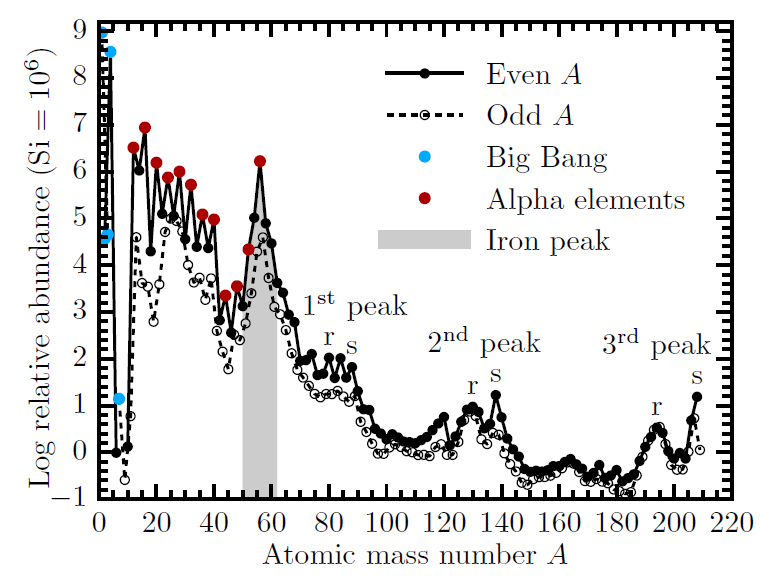
\includegraphics[width=0.25\textwidth]{./figs/intro_nuc_LipF11.png}
    \caption{
        \red{Figure from Lippuner, 1.1 TO BE Replaced}
        Figure with solar observed abundances, showing $r$-elements and $s$-elements.
        The observed obundacnes as a function of atomic mass number $A$, (data from \cite{Lodders:2003}). The plot shows nuclei that are more bound (due to \magenta{spin pairing of nucleons} \cite{Moller:1993ed}), \textit{i.e,} those with an even $A$ number, are more abundant. The lowest binding energy of nuclei with odd number of neutrons and protons (but even $A$) are largely unstable or short-lived. A few exceptions are \textit{e.g.,} $^{40}$K, $^{50}$V, $^{138}$La and $^{176}$Lu, that have a half-life of at least $10^{9}$ years.
    }
    \label{fig:intro:nuc:solar1}
\end{figure}

It was shown that the dominant nucleosynthesis process, responsible for creating elements in different mass ranges varies \cite{Burbidge:1957}. 
For instance, light elements, $A<8$, were synthesized right after the Big Bang. Nuclides before the iron peak, $12\leq A\leq 56$, come from stellar hydrostatic nuclear burning. Elements at the iron peak, $50\leq A \leq 62$, produces mostly during the type Ia supernova or explosive silicon burning in core-collapse supernova (CCSN). In these cites, the nuclear statistical equilibrium (more on that later) is established before the matter expands and cools down. 
Most of the material beyond iron peak are produced via neutron capture processes.

%%

\subsubsection{Big Bang nucleosynthesis}

The most abundant light elements in the Universe such as hydrogen, helium ($\sim 75\%$ and $\sim 25\%$ by mass), alongside trace amounts of $^{3}$He and $^{7}$Li were created during the Big Bang nucleosynthesis (BBN) (see \textit{e.g.,} \cite{Tytler:2000qf} and references therein). While involving only a small number of nuclides, the BBN is not well understood. For istance, there is a long-standing "lithium problem" \cite{Coc:2013eha}, which origin is still unclear   \cite{Fields:2011zzb}.

%%

\subsubsection{Low-mass stellar burning}

In order to fuse massive nuclides and overcome the strong Coulomb barrier, high temperatures, ($\geq 10^6$ K) are required. Thus production of heavy elements from hydrogen and helium is possible only in special environments, in particular, in the interior of stars \cite{Bethe:1939}. 

For the most of their lives stars burn hydrogen into helium. The process releases the binding energy and maintains the hydrostatic stability of a star. After the hydrogen is exhausted in the core, a core (atmosphere) contracts (expands), heats up (cools), and the shell hydrogen burning is initiated, slowly depositing ashes, \textit{e.g.,} helium, into the inert core. 
The star's subsequent evolution depends primarily on its mass. If $M>0.5M_{\odot}$, at some point the helium in the core starts to fuse into $^{12}$C and $^{16}$O and small amounts of $^{24}$Mg, $^{28}$Si. These elements are called \textit{alpha elements}  \cite{Rolfs:1988,Hasen:2004}. 

The end of the core helium burning phase leads to another core contraction phase. A star of a mass $\sim 8M_{\odot}$ would be able to ignite carbon and oxygen producing heavier elements afterwards. A less massive star looses its outer layers and becomes a slowly cooling degenerate core, a white dwarf.

%%

\subsubsection{Nuclear burning is massive stars}

A stat with the mass $M\geq 8M_{\odot}$ undergoes a sequence of burning stages  each of which leads to the exhaustion of a respective fuel, contraction of the core and rise of its temperature \cite{Woosley:2002}. 
Carbon burning leads to the production of $^{20}$Ne, $^{23}$Na and free protons that contribute to the synthesis of non-alpha elements. 
As temperature increases, the photodisintegration of $^{20}$Ne becomes possible and a small amount of $^{24}$Mg is formed. 
After that, the oxygen burning produces $^{31}$P, $^{28}$Si and $^{32}$S, that become dominant nuclides in the core by the end of oxygen burning \cite{Rolfs:1988}.

After the oxygen burning, silicon burning proceeds. The high temperatures, $T\sim3.5\times10^9$K, allow the photodissociation of some of the $^{28}$Si. This induces a sequence of alpha particle captures, "alpha ladder", on the remaining $^{28}$Si to form $^{32}$S, $^{36}$Ar, $^{40}$Ca, $^{44}$Ti, $^{48}$Cr, $^{52}$Fe and $^{56}$Ni. This process lasts around a day. \cite{Rolfs:1988,Hasen:2004}. 
Due to high temperatures preset at silicon burning, certain nuclear reactions fall into equilibrium with their inverse reactions. In particular, a quasi-equilibrium (QSE) establishes for nuclides with $A\in[28, 62]$, meaning that these nuclides (with exception of $^{12}$C, $^{16}$O $^{20}$Ne and $^{24}$Mg), are in equilibrium with each other \cite{Woosley:1973}. 

As $A=56$ the maximum binding energy per nucleon is reached, the silicon burning cannot produce heavier nuclides with the release of energy. And as the fraction of $^{56}$Ni in the core of a star increases, the support that nuclear burning provided against gravitational contraction diminishes. Meanwhile the mass of the degenerate core still increases as burning proceeds in shells.
These processes end, when the electron degeneracy pressure, that was sustaining the stellar core, can no longer counteract gravity, \textit{i.e.,} when mass of the core exceeds the effective \magenta{Chandrasekhar mass}.
%% \footnote{The collapse however occurs before the core reaches Chandrasekhar mass, and the pressure support that rests on the availability of free eletrons drops when electrons capture on the nuclides becomes possible. To account for this, the effective Chandrasekhar mass was introduced.}
Then, the core collapses, leading to a supernova (CCSN) \cite{Woosley:2002}.
During the explosion, a fraction of the mass of outer layers is ejected into the interstellar medium (ISM), enriching it with products of stellar nucleosynthesis. 

%%

\subsubsection{Iron Peak}

At temperatures higher then $T\sim 5\times10^{9}$K, \magenta{nuclear statistical} equilibrium (NSE) establishes. This is a balance between the fusion reactions forming a ($N,Z$) nuclide from $N$ neutrons and $Z$ protons and photodissociation reactions, splitting it back. 
At NSE, three parameters describe the composition: density, temperature and electron fraction, $Y_e = n_p/(n_p + n_e)$, where $n_e$ and $n_p$ are the (total) number density of electrons and protons respectively \cite{Seitenzahl:2009}. 

The composition at NSE favors more tightly bound nuclides, as they are more difficult to photodissociate. Thus, if the conditions allow, \textit{i.e.,} not too high temperature and density, and the electron fraction of the mater is $Y_e \sim 0.46$ (an electron fraction of iron), then nuclides at $A\sim56$, \textit{i.e.,} iron peak elements, dominate \cite{Seitenzahl:2009}. 
For example, NSE establishes during the type Ia supernova, when a thermonuclear explosion of a white dwarf creates right conditions for the iron peak elements to be synthesized and fall into equilibrium. After the explosion, the elements of the iron peak, as they are stable, cools and enrich the interstellar medium \cite{Iwamoto:2000as}. 

%%

\subsubsection{Nucleosynthesis beyond the iron peak}

Nuclides with $A\geq 56$ cannot be synthesized via standard cycles due to their strong Coulomb barriers. Thus, processes that do not involve charged particles become dominant. These are the neutron capture processes.
As nuclides absorb neutrons and grow larger, their binding energy $Q_n$ decreases. This process is stopped when $Q_n\sim1$MeV and energetic photons start to knock out neutrons from a nucleus. This process is called photodisintegration and a location in parameter space where it occurs, that in turn dependents on temperature and density, is called the \magenta{neutron drip line} \cite{Rolfs:1988}.

Nuclides produced via neutron capture are generally unstable to a $\beta$-decay, with a timescale $\tau_{\beta}$, that can be larger or smaller than a neutron capture timescale, $\tau_n$. 
In case when $\tau_{\beta}\ll\tau_n$, \textit{i.e.,} when a $\beta$-decay occures faster then the next neutron capture, the process is called \textit{slow} or $s$-process. 
Thus, by definition, the $s$-process moves along the valley of stability\footnote{a region of stable nuclides in the nuclides chart, a chart in terms of number of neutrons $n_n$ and number of protons $n_p$.}.
On the other hand, if $\tau_{\beta}\gg\tau_n$, \textit{i.e,} when a neutron capture occurs much faster then a $\beta$-decay, the process is called \textit{rapid} neutron capture or $r$-process. This nucleosynthesis generates nuclides near (but not crossing) the neutron drip line (see Fig.~\ref{fig:intro:nuc:srprocess}) \cite{Rolfs:1988}. 

\begin{figure}[t]
    \centering
    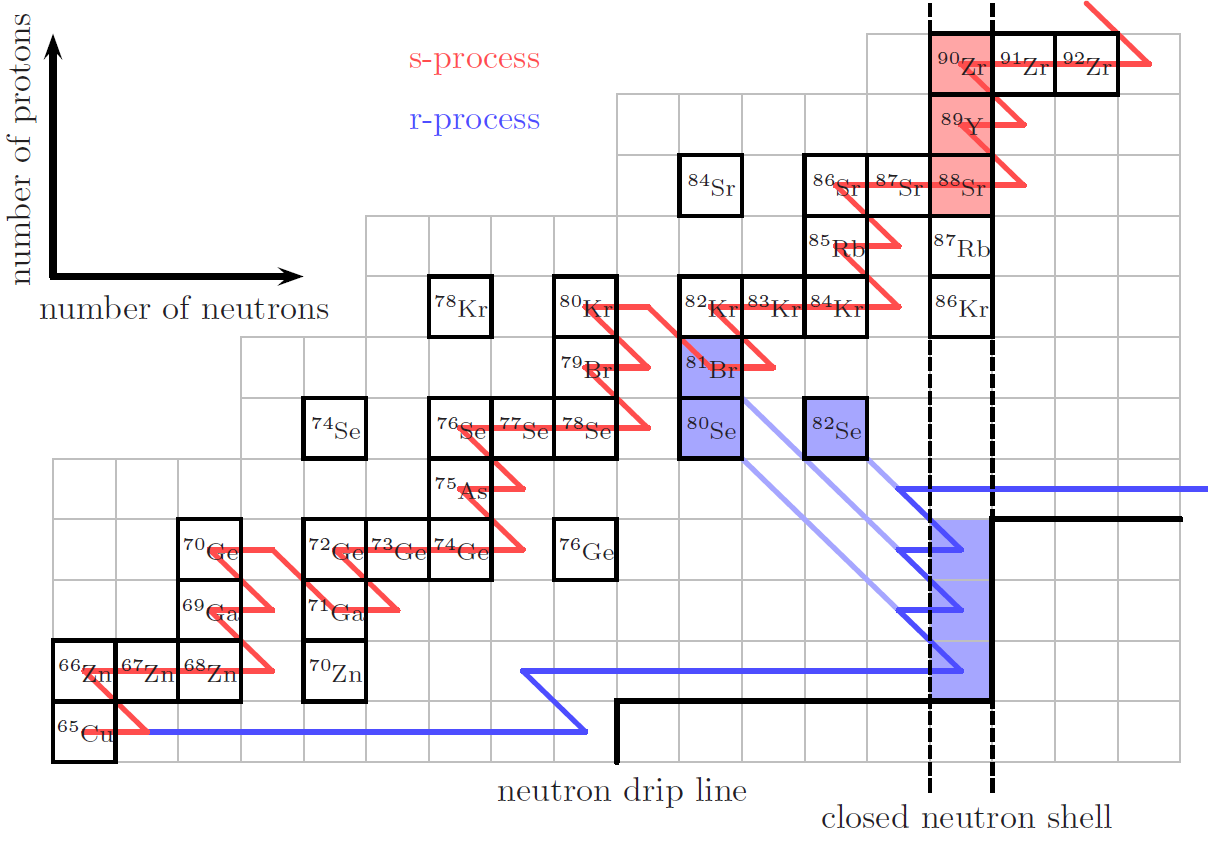
\includegraphics[width=0.25\textwidth]{./figs/intro_nuc_LipF16.png}
    \caption{
        \red{Figure from Lippuner, 1.6 TO BE Replaced}
        Schemes of $s$- and $r$-processes on a section of the nuclear chart. 
        The $r$-process runs along the neutron drip line, and the $s$-process -- along the valley of stability. 
        At a magic number, $N=50$, that correspond to the closed neutron shell, the material piles up, as the neutron capture cross-section decreases by several orders of magnitude. 
        This is the origin of the double peak structure seen in the Fig.~\ref{fig:intro:nuc:solar1}.
    }
    \label{fig:intro:nuc:srprocess}
\end{figure}

The trajectory of $r$-process is interrupted when the neutrons within nuclide can arrange themselves in a closed shell. Such configuration is energetically very favorable and thus the cross section for a subsequent neutron capture is reduced. Only after several $\beta$-decays the $r$-process continues. 
Thus, nuclides located at points where neutron drip line and closed neutron shell overlap is more abundant. These unstable nuclides will decay back to the valley of stability, some of the neutrons within them would turn to protons, reducing the total mass of the nuclide. 
The indication of this "overproduction" are the peaks in the abundance patterns at a mass, $A$, slightly lower then the one corresponding to a closed shell nuclide, Fig.~\ref{fig:intro:nuc:solar1}. 

A similar "overproduction" of nuclides with a closed neutron shell occurs when an $s$-process is considered. When the nuclides reach the closed shell, the cross-section for the next neutron capture drops, and material piles-u \cite{Rolfs:1988}. 
However, in the case of $s$-process, the peaks in abundance pattern will be at $A$, corresponding to the closed shell exactly, as the process does not wait for additional $\beta$-decays, and thus higher than $A$ of $r$-process peaks. 
Closed shell nuclides are located at $N=50,\: 82, \: 126$ and thus corresponding abundance peaks for $s$-process are at $A=88, \: 138, \: 208$ and at $A=80,\:130,\:194$ for $r$-process (see \textit{e.g.,} \cite{Arnould:2007gh}).

It was found, that the solar $r$-process abundance pattern is generic, and can be found in other places in the Universe. In particular, in stars that are formed very early, on a galactic evolution timescale. For such metal poor halo stars, one would expect to observe less $s$- and $r$-process elements as there might have been not enough time for the enrichment to take place. However recent studies showed that the solar $r$-process abundances are found in these stars as well \cite{Sneden:2008,Roederer:2010}, see also Figure 8 in \cite{Sneden:2009} 
\textcolor{red}{and section 1.9}. 

Thus, modeling the $r$-process nucleosynthesis it is expected to reproduce the solar abundances. 

It is important to mention that in addition to $s$- and $r$-process, a possible $i$-process, (intermediate) is widely discussed. 
The process operates further from the valley of stability than $s$-process, but it does not reach neutron drip line \cite{Cowan:1977,Bertolli:2013gka}. 
Slow and intermediate neutron capture processes operate within the low-mass asymptotic giant branch (AGB) stars with mass $M\in[1.5,3]M_{\odot}$ and more massive stars, that enrich the interstellar medium with heavy elements via strong winds (\textit{e.g.,} \cite{Peters:1968,Couch:1974,Kaeppeler:1994K,Woosley:2002,Straniero:2005hc,Herwig:2011}). 

%%

\subsubsection{Possible $r$-process sites}

Identification and study of possible cites of $r$-process nucleosynthesis is a rapidly developing field. Such conditions can be found in a wide variety of places, such as BBN, as models that include homogeneity suggest, neutrons star and neutron star - black hole mergers and supernova ejecta (see \cite{Mathews:1990} and references therein). 
The search for a dominant source of $r$-process nucleosynthesis is an on-going research. Spectral study of metal-poor (MP) stars, combined with models of galactic chemical evolution sheds light provide indications on what such cite might be. It is now believed that certain types of supernovae and mergers of compact objects, (NS-BH and NS-NS), are the most likely sources on $r$-process material.

\paragraph{Core-collapse supernovae}

Collapse of a massive star produces a hot neutron core, that undergoing the \magenta{deleptonization}, releases $\sim10^{53}$~erg of binding energy in form of strong neutrino flux. Irradiating dense medium around the core, these neutrinos can induce an outflow, a neutrino-driven wind \cite{Qian:1996xt}. The wind was considered as a possible cite for $r$-process \cite{Woosley:2002,Wanajo:2006mq}.
It was shown later, that the electron fraction in the wind would be too high for a full $r$-process, and only "light" heavy nuclides, up to $A\sim130$, can be synthesized \cite{Qian:1996xt,Thompson:2001ys,Fischer:2010,Roberts:2010,MartinezPinedo:2012rb,Wanajo:2013}. \textcolor{red}{add Perego:2017} 

It is important to note, in the proton-rich neutrino-driven wind nuclides with $A\sim 100$ can be produces via so-called $\nu p$-process. The process relies on the creation of free neutrons from protons via antineutrino capture. These free neutrons can then be captured by a seed nuclide $^{64}$Ge. As a result, nuclides heavier then $^{64}$Ge can be created \cite{Frohlich:2006,Pruet:2005qd,Wanajo:2010mc,Arcones:2012}.

A \magenta{full} $r$-process can be achieved in so-called \magenta{magnetorotationally driven core collapse supernovae}. This is a rare type of CCSNe, where the core of a progenitor is rotating rapidly and strongly magnetized. 
Induced by magnetorotational processes \textit{e.g.,} \magenta{magnetorotational instability}, collapse is accompanied by a formation of a collocated bipolar jet \cite{Wheeler:2000,Akiyama:2003,Burrows:2007yx,Mosta:2014jaa,Mosta:2015} \textcolor{red}{add Siegel2019?.}. 
The material in these jets is predicted to be sufficiently neutron rich to allow for a full $r$-process nucleosynthesis \cite{Winteler:2012,Nishimura:2015nca}. 
The rarity of this type of supernovae, however, might not allow it to be the dominant source or $r$-process material \cite{Nishimura:2015nca}. \red{More refs?}

%% EJECTA COMPONENTS OF BNS/NSBH MERGERS

\paragraph{Neutron star mergers}

Mergers of neutron stars, or a neutron star and a black hole have been regarded as a possible cite for the $r$-process nucleosynthesis for a long time. 
Formed in the evolution of a binary of massive stars, compact objects orbit each other for gigayears, before slow loss of energy from the system due to gravitational waves reduces their orbit and they merge \cite{Hulse:1975,Lattimer:2004sa,Price:2006fi}. 

The late inspiral and merger of binary neutron stars (BNS) or a neutron star and a black hole (NSBH) have been studied extensively via smooth particle similation \red{[REFS]} hydrodynamic simulations \red{[REFS]} and numerical relativity simulations with simplifed gravity \red{[REFS]} or full general relativity \red{[REFS]}.
\gray{For additional refs see Radice+2018ejecta paper}

%% Tidayl dynamical ejecta
These studies have shown that shortly before and during the merger, one or both compnents of the binary undergoes a tidal deformation and disruption. 
Formed streams of neutron reach matter are then ejected from the system with enough energy to be not graviationally bound to it \cite{Price:2006fi,Foucart:2014nda,Sekiguchi:2015dma,Kyutoku:2015gda,Radice:2016dwd}.
\red{More Refs from Radice/others} 

%% Shocked dynamical ejecta -> General dyanmical ejecta
In case of a BNS, when neutron stars collide, material at the collision interface, heated by shocks, gets 'squeezed out' and launched in the directions perpendicular to the plane of the binary \cite{Bauswein:2013,Hotokezaka:2013b} \red{[REFS]}. 
Generally, these tow components, tidal and shocked, constitute the \textit{dynamical ejecta}. 
The term \magenta{ejecta} referrers to the material that has enough energy to leave the system. 
The properties of the dynamical ejecta from BNS have a broad distribution, especially in terms of mass and electron fraction [\red{[REFS]} \& myFitPaper], where the former lies in range $(10^{-4},10^{-2})M_{\odot}$ and the latter $(0.05,0.45)$. 
We discuss dynamical ejecta properties of BNS in more details in section \red{sec:results:dyn\_ej:prop} and nucleosynthesis in it in the section \red{sec:results:dyn\_ej:nucleo}.

%% NSBH -- Dynamical ejecta
In case of NSBH the ejecta, only the tidal component is present. Its mass was shown to be larger, reaching $0.1M_{\odot}$ with low electron fraction, $\leq0.2$ but it requires that masses of BH and NS are comparable and BH is rapidly spinning \cite{Foucart:2014nda}\red{[REFS]}. 
If the BH is much more massive then NS, the latter would be 'swallowed' with no ejecta \red{[REFS]}.

%% Late-time ejecta
After the merger, there are expected to be additional ejecta. Consider a general postmerger configuration, consisting of a remnant (massive neutron star or a black hole), surrounded by a disk (torus) of a bounded matter. 
%% Neutrino driven wind
In case of a massive neutron star (MNS), a strong neutrino flux from the cooling remnant and the disk can drive an outflow in the direction, perpendicular to the plane of the binary, the so-called \textit{neutrino-driven wind} (see Figure 1 from \cite{Perego:2014fma}) \red{[REFS],Fujibayashi+20}. 
This ejecta is expected to occur on a timescales of $\sim100$ms postmerger, and display high eletron fraction, $Y_e\sim(0.2-0.45)$ due to neutrino irradiation and have a mass of $(10^{-4}-10^{-3})M_{\odot}$ \red{[REFS]}. 
%% Spiral-wave wind
Born in a merger, the MNS exhibit dynamical oscillations \red{[REFS]}. The $m=1$ mode, so-called "one-armed spiral instability" especially can persist on a $\sim100$ms timescale and become a dominant mode \red{[REFS], MainPaper}. 
This oscillations can inject energy into the disk, where it is carried outwards via angular momentum transport, leading to an outer part of the disk to become unbound. 
This ejecta, the \textit{\swind{}}, was shown to occur in all cases where the MNS is present is long-lived. It has high electron fraction and its mass depends on a lifetime of the remnant For a $\sim100$ms it can amount to a few $\times\sim10^{-2}M_{\odot}$ \red{[Letter, MainPaper]}. 

%% Secular ejecta
On a longer timescales, the \magenta{viscous processes} and \magenta{alpha recombination} in the disk, surrounding MNS or a BH are expected to unbind additional material. This is so-called \textit{secular ejecta}. It is expected to be massive and neutron rich. However, due to long timescales involved, it is very expensive to model \red{[REFS]}. The state of the art models involve additional assumptions, such as axisymmetry or a simplified gravity \red{[Refs]}.

%% Nucleosynthesis in Ejecta
Generally, BNS and NSBH merger ejecta is sufficiently neutron rich to allow for the $r$-process nucleosynthesis. The process can produce nuclides beyond $A=300$, which, however, are unsubtle to fission and decay. But before they reach the valley of stability they capture more free neutrons and grow again up to $A=300$ and the cycle repeats. 
This is so-called \magenta{fission cycling}. It proceeds for as long as there are free neutrons. After that, the nuclides decay to the valley of stability for the last time, forming the remarkably robust abundance pattern, independent of the number of cycles \cite{Korobkin:2012uy,Bauswein:2013,Mendoza-Temis:2014mja}, (see also Figure 4 from \cite{Korobkin:2012uy}).

\gray{We discuss the properties of the ejecta of our models and nucleosythesis within them in corresponding sections.}

%%

\subsubsection{Galactic chemical evolution}

Numerical models have shown that the final $r$-process abundances in the BNS and NSBH mergers ejecta are robust and reproduce the solar ones well \cite{Freiburghaus:1999,Goriely:2011vg,Goriely:2015fqa,Wanajo:2014,Just:2014,Radice:2016dwd}\red{[Refs]}.
The first and only so far observation of the binary neutron star merger, the event detected across all electromagnetic spectrum and in gravitational waves, cofirmed that the BNS is a cite $r$-process \red{[Refs+Strontium Ref]}.
However, the question of weather BNS (NSBH) is a dominant cite or $r$-process nucleosynthesis remains open \cite{Qian:2000bh,Argast:2003he,Matteucci:2014}. 
In particular as it is difficult to explain the observed enrichment of very metal-poor stars (MP) with $r$-process elements. In addition, the observed rather uniform $r$-process abundances in the Galaxy is not very well explained.

%% Delay
After the Big Bang nucleosynthesis, the Universe consisting of hydrogen and helium, with traces of lithium, have expanded and cooled. Under the influence of dark matter, the primordial gas fragmented, clumped and first stars, galaxies and galaxy clusters have formed. During their lifetime the first stars (population III stars) converted light elements into heavier ones and then ejected them into the interstellar medium (ISM) during supernova events. 
Future populations of stars were born of gas enriched with heavy elements, in particular, iron. Thus, the amount of elements heavier then hydrogen and helium is stars (\textit{i.e.,} metallicty) increased with each stellar generation and there exists an age-metallicity relation  \cite{Matteucci:2012}. 
Important to note, however, that multiple dark matter sub-halos contributed to the formation of the Galaxy. Thus, there might not be a unique age-metallicty relation (see \textit{e.g.,} \cite{Ishimaru:2015} and references therein).

%% Delay
The enrichment of interstellar medium with heavy elements from stellar interiors occurs immediately after stars die. However, the $r$-process elements, produced in BNS (NSBH) mergers can only enrich ISM when compact objects inspiral and merge which, on average, takes $(0.1-1)\times10^{9}$ years \cite{DeDonder:2004cx,Dominik:2012kk}. 
The exact delay time is however highly uncertain and depends on the poorly understood common envelop evolution phase of the binary (progenitors). In addition, it was shown, that a small percentage of compact binaries might form with a time delay before merger as small as $10^{6}$ years \cite{Dominik:2012kk}. 

%% Study observations
To study the chemical evolution of stars in the galaxy, the Spectroscopic surveys are conducted \cite{Edvardsson:1993,Suda:2008na}.
%% Scatter
Mergers of compact objects are rare events and thus are expected to introduce a considerable scatter into the $r$-process elements distribution in the Galaxy. However, observations show that the distribution rather uniform \cite{Argast:2003he}.
%% Scatter
It is important to note, however, that recent advances in population synthesis models, showed that with a contribution from magnetorotationally driven CCSNe the compact object mergers can account for the observed scatter of heavy elements \cite{Ishimaru:2015,Cescutti:2015,Wehmeyer:2015,VanDeVoort:2015}.

%% 244Pu
Comparison between the solar system and earth crust abundances of $^{244}$Pu have indicated that this nuclide might have been produced by rare events with high yield \cite{Wallner:2015}. This statement was confirmed via models of galactic mixing \cite{Hotokezaka:2015zea}, that also showed that there appears to be no degeneracy between rare high yields events (BNS/NSBH) and frequent low yield ones (CCSN). Similar conclusion was draws from studying $^{244}Pu$ abundances in meteorites \cite{Tsujimoto:2017}.

%% UFDG
Studies on untrafaint dwarf galaxies (UFG) also point towards rare high yield event as a prime cite of the  $r$-process nucleosynthesis. In particular, the UFG Reticulum II was shown to have a solar $r$-process abundances, while UFG of similar type tend to have $2-3$ times less $r$-process elements. This suggests that a rare high-yield event has modified Reticulum II chemical composition, and high europium abundances indicate that it was a compact object merger \cite{Ji:2016}. 

Thus, it is still unclear whether the observed degree of homogeneity in $r$-process elements distribution in the galaxy and $r$-process elements enrichment of VMP stars can be explained BNS or NSBH mergers.

\red{Mention Actinide abundaces problem.}


%%

\subsubsection{Kilonova}

Nuclides, synthesized in $r$-process are very neutron rich and unstable. 
After the last fission cycle, they decay to the valley of stability. This process takes from hours to days and released energy that can power an electromagnetic transient, called Kilonova or Macronova 
(\textit{e.g.,} \cite{Li:1998bw,Kulkarni:2005jw,Metzger:2010,Roberts:2011,Metzger:2016pju,Wollaeger:2017ahm})\red{more refs}

\gray{
In 2017 such electromagnetic signal, AT2017gfo after the gravitational wave, GW170817, one 
confirmed that indeed, $r$-process nucleosynthesis takes place in the ejecta from merger of compact objects, in that case of two neutron stars [REFS]. 
}

% [RED]
Kilonova has a complex observational signature due to different ejecta components with various compositions contribution to it. 
In particular, it was shown that if produced, lanthanides, $(58\leq Z \leq71)$, and actinides, $(90\leq Z \leq 103)$, that have an open $f$-shell and hence a very large number of absorption lines, increases the opacity of emitting region by a factor of $10$. These elements are produced only if electron fraction of the ejecta was sufficiently low, $Y_e\leq 0.25$, \cite{Lippuner:2015gwa}. Such low $Y_e$ is present for instance in a tidal component of dynamical ejecta. 
High opacity of the emitting region implies that a transient is dim, $(\sim10^{40})$ erg s$^{-1}$, and peaks around a weak after merger in the red/infrared band \cite{Barnes:2013wka,Grossman:2013lqa,Lippuner:2015gwa}. 

% [BLUE]
If the ejecta electron fraction is high, $Y_e \geq 0.25$, weak $r$-process would produce a small amount of lanthanides, and the opacity of the emitting region thus would be lower. The kilonova signal originating from such ejecta would be bright and peak on a timescale of a few days in a blue band \cite{Kasen:2014toa,Martin:2015hxa}. 

\gray{
Indeed, both blue and red components were observed in the case of AT2017gfo, that confirmed the general picture \red{[Villar2017]}. However, estimated mass of the ejecta required to explain the red component is larger then what is predicted by numerical relativity simulations \red{refs}. It is believed that the most contribution to this component comes from the low $Y_e$, slow but massive outflow from the degenrate disk on a secular timescale \red{refs}.
}

In addition to aforementioned electromagnetic signals, a very short, bright ultraviolet precursor can be produced. It originates from high velocity tale of the dynamical ejecta, where neutrons might avoid being captuired on a seed nuclide and freely decay \cite{Metzger:2014yda}. 
\gray{
Unfortunately, in case of AT2017gfo, the electromagnetic followup started \red{11} hours after the gravitation wave detection.
}
See Figure 6 from \cite{Metzger:2016pju} for an examples of lightcurves of Kilonova and precursor.

The search for electromagnetic counterparts to mergers continues, involving observatories around the world \cite{Law:2009,Singer:2014qca,Bellm:2014,Kasliwal:2016uhu}.

%%

\subsubsection{Non-thermal emission}

% EJECTA
A very high energy emission from the non-thermalized radiation is weak and can be detected only for a sufficiently close event \cite{Hotokezaka:2015cma}.

% GRB
\red{Subsection of GRBs}
\cite{Lee:2007js,Nakar:2007yr,Gehrels:2009,Fernandez:2015use}

%%
%%
%%

\subsection{Modeling the $r$-process nucleosynthesis}

Nucleosynthesis calculations are of utmost importance for a large number of astrophysical applications. Nuclear burning withing the main sequence stars \cite{Bethe:1939} creates elements up to iron group. Explosive synthesis withing a supernova generates iron-group elements and beyond with contributions from $s$-process \cite{Burbidge:1957}, and weak $r$-process \cite{Wanajo:2013}. Elements, that ultimately enrich the ISM \cite{Nomoto:1997if,Woosley:2002}. In BNS and NSBH mergers, the full $r$-process nucleosynthesis is believed to be possible \cite{Freiburghaus:1999}, synthesizing the heaviest elements, lanthanides and actinides [Refs].

To model the aforementioned processes is it necessary to compute nuclear reactions and not only focusing on the total energy generation (\textit{e.g.,}  \cite{Weaver:1978,Mueller:1986,Timmes:1999}) but tracking the evolution of the whole ensemble of nuclear species \red{[Refs]}.
A mathematical and/or numerical model that describes coupled nuclear reactions, tracking the evolution of abundances of various species, coupled by a non-liear reaction rates is called \textit{nuclear reaction network} (NRN).

The complexity of networks, \textit{i.e.,} the number of species and reactions evolved, varies depending on the intended implementation.
%% BBN
For instance, for a Big Band nucleosynthesis rarely more then a dozen nuclear species are evolved 
\cite{Wagoner:1973,Orlov:2000,Nollett:2000fh,Coc:2013eha,Cyburt:2015mya}. 
%% STellar
To model nucleosynthesis in stars tens or even hundreds of them are used in a more recent and advanced models \cite{Arnett:1977,Weaver:1978,Paxton:2011,Bressan:2012,Jones:2015}
%% SN
Networks designed for explosive nuclear burning and supernovae have come a long way from including only a few tens of species (\textit{e.g.,} \cite{Truran:1966,Truran:1967,Arnett:1969,Woosley:1973}) to including hundreds of species and reactions, (\textit{e.g.,} in type Ia SN \cite{Thielemann:1986,Hillebrandt:2013gna,Seitenzahl:2013,Leung:2015fxa}, in core-collapse supernovae \cite{Thielemann:1986,Limongi:2003ui,Heger:2008td,Harris:2014}, in novae \cite{Weiss:1990,Jose:1997vf,Iliadis:2002zz,Starrfield:2016} and X-ray bursts \cite{Schatz:2001xx,Woosley:2003cd,Cyburt:2010,Parikh:2012hx}) 
%% r-process
Neutron captures result in a formation of unstable nuclides, that decay via extensive chains of reactions, involving hundreds and thousands of steps. Thus, nuclear reaction networks has to be adequately complex to model the $s$-process, (\textit{e.g,} \cite{Prantzos:1990,Kaeppeler:2011,Nishimura:2017zdi}) and even more so to model $r$-process. 
The applications of such NRN are vast. In CCSN neutrino driven winds (\textit{e.g.,} \cite{Woosley:1992,Arcones:2010,Wanajo:2013}).
In outflows from magnetorotational CCSN (\textit{e.g., \cite{Winteler:2012,Nishimura:2015nca}}. 
In compact object mergers several cites with different conditions require modeling. 
In particular, in dynamical ejecta \cite{Goriely:2011vg,Bauswein:2013,Wanajo:2014,Just:2014,Fernandez:2016sbf}\red{[Refs]}, in the disk (torus)  \cite{Surman:2008qf,Perego:2014fma,Martin:2015hxa,Lippuner:2017tyn}\red{[Refs]}. And these are only selected examples of where modeling of neutron capture nucleosynthesis is done. See \cite{Blinnikov:1996,Panov:1995,Panov:2001,Mumpower:2011ar}\red{[Refs]} for overview.

%% modelling the network
Key components of a NRN are interactions between two and more nuclides, catheterized by reaction rates (RR), as well as single particle reactions, such as $\beta$-decay.
Reactions between charged particles require that the Coulomb barrier is overcome. Thus, in general, RR depend strongly on the particle energy as well as on \magenta{resonances} in compound nuclear systems (\textit{e.g.,} \cite{Clayton:1968}, \textsection{4}). 
\gray{ %% Additional, not crucual information
In single-particle reactions, \textit{e.g.,} $\beta$-decay, it is common to assume a constant RR, which is strictly speaking is true only in vacuum. 
Another common approach to treating complex reactions, is to assume that reactants form a single nuclide that undergoes a chain of decays into reaction products. This is called a Hauser-Feshbach approach. It is particulalrly useful for reactions far from the valley of stability with a long chains of decay \cite{Hauser:1952,Rauscher:2000fx,Goriely:2008zu}. 
In addition, in order to model the nuclear statistical equilibrium (NSE) and $\beta$-decay rates, nuclide masses and partition functions (\cite{Arcones:2010dz,Brett:2012jn,Mendoza-Temis:2014mja,Mumpower:2015ova}) have to be prescribed. 
This data is not fully available and have large uncertainties (see \textit{e.g.,} \cite{Lunney:2003,Schatz:2013,Mumpower:2015ova} and references therein). 
Thus, often theoretical models for nuclear masses and $\beta$-decay properties are used for many species \cite{Lunney:2003,Moller:2003,Mumpower:2015ova}. 
}

Several nuclear reaction networks are available in the literature. 
In particular: 
a set of networks by \cite{Timmes:1999} \footnote{\url{http://cococubed.asu.edu/code_pages/burn.shtml}}, 
\texttt{XNet} by \cite{Hix:1999} \footnote{\url{http://eagle.phys.utk.edu/xnet/trac}} , 
\texttt{NucNet} by \cite{Meyer:2007} and a  \footnote{\url{https://sourceforge.net/projects/nucnet-tools}}
\texttt{SkyNet} by \cite{Lippuner:2015gwa} \footnote{\url{https://bitbucket.org/jlippuner/skynet}}.

In this thesis we employ \texttt{SkyNet} to compute nucleosynthetic yields in binary neutron star mergers ejecta. 
We introduce the NNR in the follwing subsection and discuss its main advantages. 
\texttt{Skynet} is a modular and versatile nuclear reaction network designed initially for $r$-process nucleosynthesis calculations. It is capable of evolving arbitrary set of nuclear
species in NSE as well as switching to a full network self-consistently. The network incorporates \magenta{screening corrections} and equation of state that considers an entire composition. 

\texttt{SkyNet} is a popular choice for studying nucleosynthesis in neutron rich environment \cite{Lippuner:2015gwa,Radice:2016dwd,Roberts:2016igt,Lippuner:2017tyn,Siegel:2017nub,Vlasov:2017nou,Fernandez:2016sbf} \red{[Refs(us,david)]}, .

%%
%%
%%

\subsubsection{Nuclear reaction network basics}
\red{This might go into TheoryAppendix}

Nuclear reaction networks allow to track the evolution of a system of many nuclear species that undergo transmutations in prescribed reactions given the reaction rates. 
The rate equations describe microscopic processes. They are based on the kinetic theory. For instance, a system of non-correlated particles, involved in interactions, some of which can change particle type, can be described in terms of a distribution function. 
The evolution of this function is given by Kinetic theory \red{Danielewicz and Bertsch, 1991; Buss et al., 2012}. 

Generally, only a subset of particles is evolved by a NRN, while for others the conditions are assumed to be constant. 
For instance, \magenta{photons are generally assumed to be in equilibrium} at all times, while electron and positron densities are set by the \magenta{charge neutrality}. 

% Abundances
When describing particle interactions and nuclide transmutations it is common to introduce the entrance and exit channels representing reactants and products. 
Then, a reaction rate is defined as a speed at which a reaction proceeds per particle in the entrance channel. It follows then that, if there is no change between particles in entrance and exit channels, the RR is zero. 
A particular useful quantity is \textit{abundance} $Y_i$, defined as 

\begin{equation}
\label{eq:theory:nuc:abundance}
Y_i = \frac{n_i}{n_B} = \frac{N_i/V}{N_B/V} = \frac{N_i}{N_B},
\end{equation}

where $V$ is the volume of the fluid element, $N_i$ and $N_B$ are the total numbers of particles of species $i$ and baryons respectively. It is usually abundances of $Y_i$ that are evolved in nuclear reaction networks instead of particle number densities $n_i$ as the latter depend on the volume that often is not constant. 
The abundance evolution equation reads

\begin{equation}
\frac{\text{d}Y_i}{\text{d}t} = \sum\lambda_{\alpha}(-R_{i}^{\alpha}+P_{i}^{\alpha})N_{i}^{\alpha}\prod_{m\in\mathcal{R}_{\alpha}}Y_m^{N_{m}^{\alpha}}
\end{equation}

where $\lambda_{\alpha}$ is the reaction rate of the forward process, $R_{i}^{\alpha}$ are reactants, $P_{i}^{\alpha}$ are products, $N_{i}^{\alpha}$ number of particles of the species $i$ involved and $Y_m^{N_{m}^{\alpha}}$ are the abundances of the particles of psecies $i$ involved (see e.g., \cite{Hix:1999}).

The \texttt{SkyNet} solves the coupled first-order non-linear system of equation, \eqref{eq:theory:nuc:abundance}, for a given set of reaction rates $\lambda_{\alpha}$.
The Eq.~\eqref{eq:theory:nuc:abundance} can be understood as following. The time derivative of the species $i$ abundances is given by the sum over all reactions, in which the species in question participate. 
Each reaction contribution consists of multiplies: reaction rate, a factor describing creation or destruction of particles (of species $i$), \textit{i.e.,} the number of particles, and abundances of reactants.

A representative example is carbon burning $^{12}\text{C} + ^{4}\text{He} \leftrightarrow ^{16}\text{O}$:

\begin{eqnarray*}
    \frac{\text{d}Y^{12}\text{C}}{\text{d}t} &= -\lambda_{\alpha}Y_{^{12}\text{C}} Y_{^{4}\text{He}} + \lambda_{\alpha'}Y_{^{16}\text{O}} + \dots , \\
    \frac{\text{d}Y^{4}\text{He}}{\text{d}t} &= -\lambda_{\alpha}Y_{^{12}\text{C}} Y_{^{4}\text{He}} + \lambda_{\alpha'}Y_{^{16}\text{O}} + \dots , \\
    \frac{\text{d}Y^{16}\text{O}}{\text{d}t} &= \lambda_{\alpha}Y_{^{12}\text{C}} Y_{^{4}\text{He}} + \lambda_{\alpha'}Y_{^{16}\text{O}} + \dots . \\
\end{eqnarray*}

%%

\paragraph{Reaction rates and velocity averaged cross-sections}

%% ---------------
%%
%% References
%%
%% ---------------

\newpage

\bibliography{../references}


\end{document}
